\documentclass[
candidate, % тип документа
subf, % подключить и настроить пакет subfig для вложенной нумерации рисунков
%href, % подключить и настроить пакет hyperref
%colorlinks=true % цветные гиперссылки
times % шрифт Times как основной
%,fixint=false % отключить прямые знаки интегралов
]{disser}

%\renewcommand{\rmdefault}{ftm}
\usepackage{tempora}


%\usepackage[nodisplayskipstretch]{setspace}
%\onehalfspacing
%\parskip 1.5ex % paragraph spacing

\usepackage[
a4paper, mag=1000,
left=3cm, right=1.5cm, top=2cm, bottom=2cm, headsep=0.7cm, footskip=1.25cm
]{geometry}



\usepackage[T2A]{fontenc}

\usepackage[utf8]{inputenc}
\usepackage[english,russian]{babel}

%\usepackage{paratype}
%\defaultfontfeatures{Ligatures={TeX},Renderer=Basic} 
%\setmainfont[Ligatures={TeX,Historic}]{Times New Roman}
\usepackage{pdfpages}
\ifpdf\usepackage{epstopdf}\fi

\usepackage{dcolumn}
\usepackage{bm}
\usepackage{hyperref}
\usepackage{color}
\usepackage{epstopdf}
\usepackage{amsmath}
\usepackage{amssymb}
\usepackage{cite}
\usepackage{multirow}
\usepackage{afterpage}
\usepackage[font={normal}]{caption}
%\usepackage{setspace}
\usepackage{amsmath} % align
\usepackage[onehalfspacing]{setspace}% 1,5 интервал
%\usepackage{biblatex}
\usepackage{fancyhdr} % пакет для установки колонтитулов
\pagestyle{fancy} % смена стиля оформления страниц
\fancyhf{} % очистка текущих значений
\fancyfoot[C]{\thepage} % установка верхнего колонтитула
\renewcommand{\headrulewidth}{0pt} % убрать разделительную линию

\usepackage{caption} % подписи к рисункам в русской типографской традиции
\DeclareCaptionFormat{GOSTtable}{#2#1\\#3}
\DeclareCaptionLabelSeparator{fill}{\hfill}
\DeclareCaptionLabelFormat{fullparents}{\bothIfFirst{#1}{~}#2}
\captionsetup[table]{
	format=GOSTtable,
	%font={footnotesize},
	labelformat=fullparents,
	labelsep=fill,
	labelfont=it,
	textfont=bf,
	justification=centering,
	singlelinecheck=false
}

\usepackage{amsmath,amssymb}
\captionsetup{format=hang,labelsep=period}

% Использовать полужирное начертание для векторов
\let\vec=\mathbf

% Включать подсекции в оглавление
\setcounter{tocdepth}{2}

\graphicspath{{img/}}


\pagestyle{footcenter}
\chapterpagestyle{footcenter}

% Подсветка кода
\usepackage{pythonhighlight}

% Для приложений А3 формата
\usepackage[paper=A4]{typearea}
\begin{document}
	%\includepdf[pages={1-1}]{Titul_vkr.pdf}
	% Содержание
	
	%\chapter*{Введение}
%\addcontentsline{toc}{chapter}{Введение}

\newpage
\begin{center}
	\textbf{АННОТАЦИЯ}
\end{center}
%\refstepcounter{chapter}
\addcontentsline{toc}{chapter}{АННОТАЦИЯ}

Целью данной работы является разработка более доступного и дешевого четвероногого робота для образовательных и исследовательских целей. Лучшая доступность достигается путем проектирования робота таким образом, чтобы его можно было собрать без каких-либо специальных инструментов, а все необходимые детали были либо напечатаны на 3d-принтере, либо легко изготовлены. Для снижения стоимости, вместо дорогих бесщеточных двигателей и контроллеров двигателей используются доступные сервоприводы. Для того чтобы конструкция робота была полезна для образования и исследований, она должна обладать большинством возможностей более крупных и дорогих экземпляров. Это достигается путем изучения существующих конструкций четвероногих роботов и выбора возможных компромиссов.

Конечная цель - разработать подходящую структуру управления, которая обеспечит автономную работу робота для демонстрации возможностей аппаратного обеспечения.

В данной работе достигнуты следующие цели:
\begin{enumerate} 
	\item Решены задачи траекторного движения на основе численного решения обратной задачи кинематики.
	\item Спроектированы твердотельные чертежи и произведена сборка физической единицы робота.
	\item Разработана модель движения робота с учетом обратной связи, основанной на данных с инерционного датчика.
\end{enumerate}
Результат работы представлен в виде работоспособного физического прототипа шагающего робота с возможностью дистанционного управления.


\onehalfspacing
\setcounter{page}{2}
\renewcommand{\contentsname}{\centerline{\Large{Cодержание}}}
\tableofcontents
\addtocontents{toc}{\protect\thispagestyle{fancy}}
\renewcommand{\contentsname}{\centerline{\Large{Cодержание}}}

\newpage
\begin{center}
	\textbf{ВВЕДЕНИЕ}
\end{center}
%\refstepcounter{chapter}
\addcontentsline{toc}{chapter}{ВВЕДЕНИЕ}

Особенное место в робототехнике занимает подкласс шагающих роботов. Шагающими роботами принято называть класс роботов, которые имитируют походку людей или животных. Данный вид появился не просто так, их главной особенностью является как особенность походки, так и в принципе уникальная модель движения. Она позволяет быстро и, что главное, эффективно приспосабливаться к работе в неровных поверхностях\cite{movement_art}. По сути, оптимизация движения шагающих роботов является главной проблемой всех ведущих исследователей в данной области. Все известные производители шагающих роботов не используют четко описанные законы движения для управления в своих продуктах. Вместо этого, они используют заранее сформированные модели глубокого обучения, основанные на больших пластах информации, собранной с реальных экземпляров. Например, для управления (обучения) четырехногих шагающих роботов использовали массивы данных, полученных с датчиков, которые в свою очередь были закреплены на собаке, схожей по физическим размерам конечностей и тела\cite{dog_and_robo_dog}. Такие методы, как правило показывают себя более выгодными как с точки зрения точности позиционирования робота, скорости адаптации в окружении, так и выигрывают по энергоэффективности в сравнении с классическими методами, но имеют существенный недостаток в скорости разработки и в особенности требуют больших денежных затрат. 
\newpage
\textbf{Актуальность}


Задача разработки шагающих роботов не теряет актуальности по сей день. Начиная с 2004 года, когда Boston Dynamics впервые представила четырехногого шагающего робота BigDog, промышленность в данной области не сбавляет обороты и постоянно вносит новые технологии, методики в разработку, а также находит новые применения данным роботам. Прогресс можно заметить при сравнении с современными моделями Boston Dynamics или, например LaikaGo и Strelka от UniTree\cite{Laika}  (рисунок \ref{dogs}), которые используют на кафедре робототехники в МГТУ им. Н. Э Баумана.
\begin{figure}[h]
	\begin{center}
		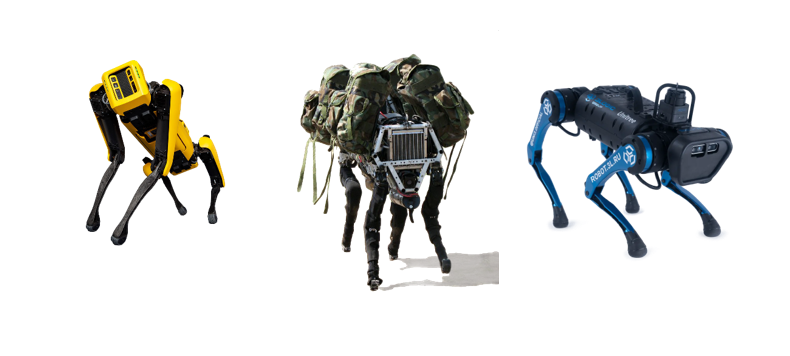
\includegraphics[width=1\textwidth]{dogs}
		\caption{BigDog и Spot от Boston Dynamics, Laika от UniTree}
		\label{dogs}
	\end{center}
\end{figure}

Сегодня такие мобильные роботы используются для составления строительных планов здания по технологии BIM (рисунок \ref{zavod}), отслеживания хода строительства на площадках Pomerlau, а также на заводах Ford. Такие продукты стали востребованы для мониторинга оборудования в опасных условиях, например, нефтепромышленная компания AkerBP использовала робота Spot для снятия показаний и отслеживания утечек на судне FPSO в Норвегии\cite{fpso1,fpso2}.

\newpage
\begin{figure}[h]
	\begin{center}
		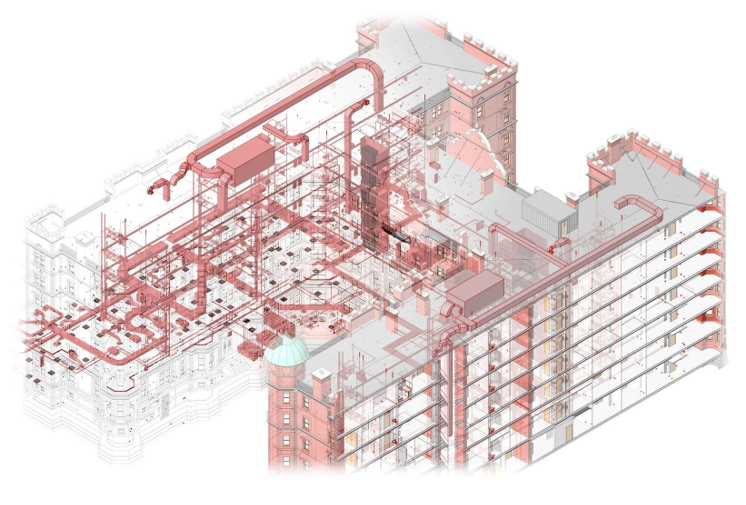
\includegraphics[width=1\textwidth]{zavod}
		\caption{Строительный план по технологии BIM}
		\label{zavod}
	\end{center}
\end{figure}
	\newpage
	

\newpage
\begin{center}
	\textbf{\large ГЛАВА 1 \\ ПОСТАНОВКА ЗАДАЧИ И ПЛАН РЕШЕНИЯ}
\end{center}
\refstepcounter{chapter}


% \section*{}
\addcontentsline{toc}{chapter}{ГЛАВА 1}
\section{Анализ существующих моделей шагающих роботов}

Автономных роботов можно условно разделить на две категории: стационарные роботы и мобильные роботы. Одним из типов стационарных робототехнических систем является манипулятор, который размещает поверхностно установленные компоненты с чрезвычайно высокой точностью\cite{bibl1}, т.е. в сборочной линии, рука робота способна перемещаться с высокой скоростью и точностью для выполнения повторяющихся задач, таких как точечная сварка\cite{welding} и покраска\cite{painting}.

Другим важным типом стационарных роботизированных систем является устройство схвата\cite{grab}, которое обычно используется для захвата нужных объектов. В настоящее время разработано множество роботизированных механических устройств имитирующие руки и пальцы, которые широко применяются,например, в сельском хозяйстве\cite{farming}. К сожалению, эти стационарные роботы страдают от недостаточной подвижности и ограниченного диапазона движения. В отличие от них, мобильные роботы способны передвигаться по пересеченной местности. Благодаря гибкости мобильных роботов, они широко применяются во многих областях, таких как строительство, охрана объектов, сбор информации. В этих сценариях применения мобильные роботы могут быть классифицированы на наземные, воздушные и подводные. Кроме того, в соответствии с различными механическими структурами, наземных роботов можно разделить на колесные, гусеничные и шагающие роботы, соответственно.

На неровной местности для перемещения больше подходят шагающие роботы, в силу их способности адаптироваться к местности. Кроме того, они также могут применяться областях, далеких от промышленности, например медицина \cite{medicine1,medicine2} и образование \cite{edu}. Таким образом, шагающие роботы стали актуальной темой для исследований в области робототехники, благодаря их преимуществу перед колесными и гусеничными роботами.

Рассмотрим несколько моделей шагающих роботов, на основе которых проведем анализ конструкции (раздел \ref{C1_2}).

Mini Cheetah \cite{cheetah} --- это четырехногий робот, разработанный в Массачусетском технологическом институте (рисунок \ref{cheetah}). Основное внимание в роботе уделяется его модульным приводам высокой мощности. Mini Cheetah обладает двенадцатью одинаковыми приводами, которые состоят из бесщеточного двигателя, планетарного редуктора с передаточным числом 6:1, энкодера и контроллера двигателя. Все приводы Mini Cheetah обмениваются данными по единой шине CAN-bus.
\begin{figure}[h!]
	\begin{center}
		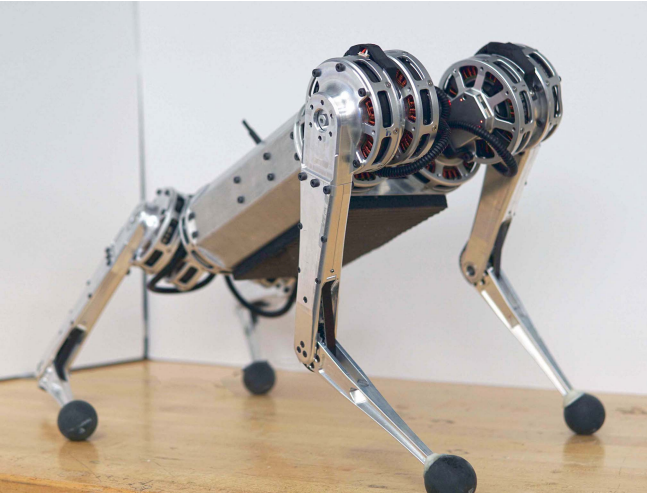
\includegraphics[width=0.5\textwidth]{cheetah}
		\caption{Mini Cheetah, разработанный в MIT}
		\label{cheetah}
	\end{center}
\end{figure}

Stanford Doggo\cite{SDoggo} --- квази-прямоходящий четырехногий робот, разработанный в Стэнфорде. Квази-прямоходящий - термин, описывающий движение, которое почти прямолинейно, но с некоторой степенью отклонения от прямой линии. Данный робот обладает очень высокой выходной мощностью по сравнению с его весом и низкой ценой. Такой высокий крутящий момент достигается за счет квазипрямого привода и меньшего количества степеней свободы на каждой ноге.
\newpage
\begin{figure}[h!]
	\begin{center}
		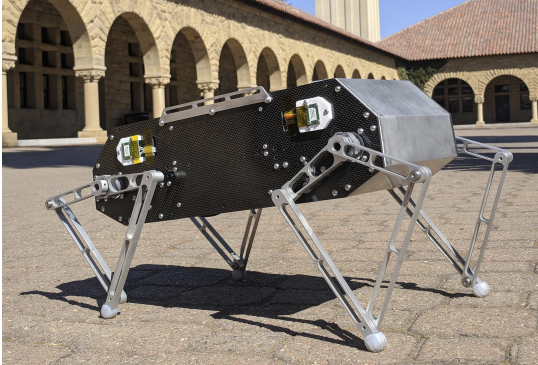
\includegraphics[width=0.5\textwidth]{SDoggo}
		\caption{Stanford Doggo, разработанный в Стэнфордском университете}
		\label{SDoggo}
	\end{center}
\end{figure}

Spot\cite{spot} --- шагающий робот, разработанный компанией Boston Dynamics, представляет из себя четвероногого робота, предназначенного для промышленного рынка. По этой причине он обладает более широкими возможностями, чем другие четвероногие роботы, так как создан для выполнения бизнес задач. Он обладает хорошей подъемной силой, имеет возможность установки дополнительных датчиков и инструментов на верхней части корпуса, а также использует камеру для технического зрения с целью сканирования окружающей обстановки.%\comment{ ОБЗОР ПО НАУЧНЫМ ИССЛЕДОВАНИЯМ}{comment}
\begin{figure}[h!]
	\begin{center}
		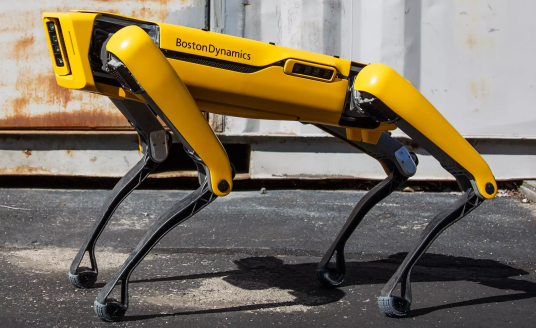
\includegraphics[width=0.5\textwidth]{spot}
		\caption{Spot, разработанный в компании Boston Dynamics}
		\label{spot}
	\end{center}
\end{figure}


\section{Задачи работы}\label{C1_1}

Создание функционирующего прототипа шагающего робота, приближенного к промышленным моделям, является существенно сложным и дорогостоящим процессом. В связи с этим, для достижения поставленных целей, в данной работе будут применены упрощения, которые окажут влияние на некоторые технические аспекты, однако не повлекут за собой потерю общей ценности исследования - разработки действующего прототипа с готовым управлением, полученным путем решения задач механики и управления без использования методов искусственного интеллекта.


%Задача создания работоспособного прототипа шагающего робота близкого к промышленным образцам является очень сложной и одновременно дорогостоящей работой. По этой причине в рамках работы будут использоваться упрощения, которые повлияют на некоторые технические особенности, но не изменят общей ценности работы – разработки работоспособного прототипа с готовым управлением, полученным путем решения задач механики и управления без применения искусственного интеллекта.
 
Для выполнения данного проекта потребуется выполнить следующие работы:
\begin{enumerate}
	\item Разработать кинематическую схему ноги робота.
	\item Разработать общую кинематическую схему робота.
	\item Решить обратную задачу кинематики для положения ноги.
	\item Решить задачу описания модели походки робота.
	\item Разработать твердотельную модель ног и корпуса робота.
	\item Подобрать необходимые сервоприводы в сочленения ног робота.
	\item Подобрать комплектующие, связанные с реализацией контроля сервоприводами.
	\item Разработать программное обеспечение для дистанционного управления роботом.
	\item Автоматизировать внутренние процессы прототипа. 
	\item Создать графический интерфейс для управления.
\end{enumerate}
В настоящей работе будут тщательно рассмотрены пункты \textbf{1-6} и описаны пункты \textbf{7-8} , пункты \textbf{9-10} рассматриваться не будут.
\section{Исследование особенностей конструкции робота}\label{C1_2}
Среди всех компонентов робота, ноги являются наиболее важными составляющими. Такие свойства, как вес, размеры и приведение в действие суставов, непосредственно влияют на производительность движения ног и, следовательно, точность позиционирования робота.

У упомянутых ранее моделей роботов схожи комплекции как корпуса, так и ног, даже общие объемы роботов будут схожи. 
Каждая нога состоит из тазобедренного сустава, бедра, коленного сустава, голени и стопы для контакта с землей, то есть все ноги обладают тремя степенями свободы, а принципы расположения двигателей в ногах имеют минимальное расхождение. Это следствие того, что промышленные модели сделаны из металла и действительно требуют расположения тяжелых двигателей как можно ближе к корпусу для большей устойчивости и меньших затрат на управление. 

В данном проекте робот не обладает существенным весом, а также большими размерами корпуса и ног, в следствие чего будут следующие упрощения:
\begin{itemize}
	\item На одну ногу приходится две степени свободы, вместо распространенной схемы в виде трех степеней.
	\item Двигатели располагаются в области бедра (у корпуса) и колена (в сочленении ног), так как робот обладает небольшой массой и малыми габаритами для классического решения (рисунок \ref{kinematic}).
\end{itemize}


Указанные упрощения могут привести к утрате возможности контролировать отклонения бедра, что в свою очередь подчеркивает необходимость разработки методов компенсации устойчивости при изменениях углов ориентации корпуса в плоскостях крена и тангажа.
\newpage
\begin{figure}[h]
	\begin{center}
		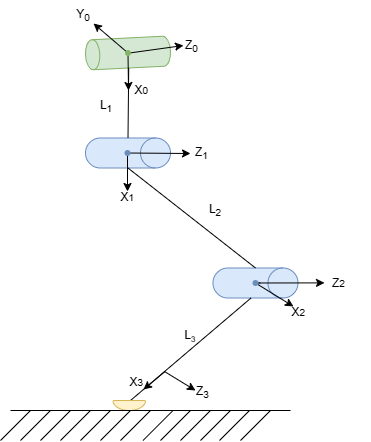
\includegraphics[width=0.6\textwidth]{kinematic}
		\caption{Расположения двигателей для случая трех степени свободы на ногу}
		\label{kinematic}
	\end{center}
\end{figure}

	\newpage
	
\newpage

\begin{center}
	\textbf{\large ГЛАВА 2 \\ КИНЕМАТИЧЕСКАЯ СХЕМА РОБОТА}
\end{center}
\refstepcounter{chapter}


% \section*{}
\addcontentsline{toc}{chapter}{ГЛАВА 2}
\section{Общая схема робота}\label{C2_1}

 %В главе \ref{C1_2} были получены требования к кинематической схеме робота. Необходимо разработать прототип ноги, который представляет из себя двухзвенный механизм с двумя двигателями. Один двигатель расположен ближе к корпусу робота и отвечает за ориентацию положения первого звена, имитирующее бедро робота. Второй двигатель связывает первое и второе звено, которое в свою очередь имитирует голень робота, а также обладает подобием стопы на конце. Конечная кинематическая схема ноги приведена на рисунке \ref{Areaconfig} 
В разделе \ref{C1_2} были определены требования к кинематической конфигурации робота. В целях создания прототипа ноги предложена двухзвенная механическая система, оснащенная двумя двигателями. Первый двигатель расположен ближе к корпусу робота и обеспечивает ориентацию положения первого звена - имитации бедра робота. Второй двигатель связывает первое и второе звено, которое, в свою очередь, имитирует голень робота и завершается элементом, аналогичным стопе. Результирующая кинематическая схема ноги представлена на рисунке \ref{kinematic2D}.

\begin{figure}[ht]
	\begin{center}
		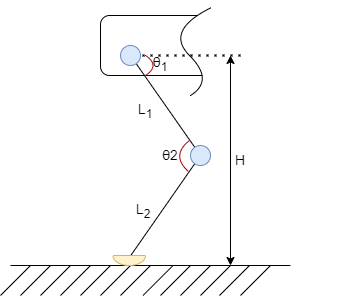
\includegraphics[width=0.5\textwidth]{kinematic2D}
		\caption{Кинематическая схема ноги робота}
		\label{kinematic2D}
	\end{center}
\end{figure}

%Таким образом робот имеет четыре одинаковые ноги. Они прикреплены к туловищу таким образом, что шарнирные соединения передних и задних ног обращены друг от друга, как показано на рисунке 2.2. Каждая нога имеет две степени свободы, одна которых лежит на плечевой части (тазобедренный сустав) и одна на коленном суставе. 
Таким образом, робот имеет четыре одинаковые ноги, каждая из которых имеет две степени свободы. Шарниры передних и задних ног направлены в противоположные стороны и закреплены на туловище, как показано на рисунке \ref{full}. Степени свободы распределены между плечевой частью (тазобедренный сустав) и коленным суставом.

\begin{figure}[h!]
	\begin{center}
		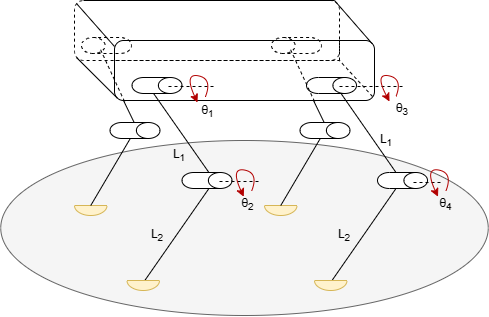
\includegraphics[width=0.8\textwidth]{full}
		\caption{Полная кинематическая схема робота}
		\label{full}
	\end{center}
\end{figure}

\section{Построение рабочей области ноги робота}\label{C2_2}
Для того, чтобы решить обратную задачу кинематики, необходимо определять положения углов с течением времени для совершения шага по некоторой траектории, следовательно, необходимо понимать рабочую область исследуемого объекта, в данном случае ноги. Общие характеристики ноги сведены в таблице \ref{tablParam}


\begin{table}[h]
	\begin{center}
		\caption{Характеристики ног робота}
		\label{tablParam}
		\begin{tabular}{| l | l |}
			\hline
			Общий вес   &    0.2 кг \\ \hline
			Длина первого звена & 100 мм\\ \hline
			Длина второго звена & 100 мм \\ \hline
			Диапазон поворота двигателя (бедро) & $\pm$ 180$^{\circ}$ \\ \hline
			Диапазон поворота двигателя (колено) & $\pm$ 180$^{\circ}$ \\ \hline
		\end{tabular}
	\end{center}
\end{table}

Чтобы описать рабочую область, составим кинематическую схему, представленную на рисунке \ref{Areaconfig} и решим задачу о положении стопы ноги. Точку O будем считать зафиксированной на корпусе. 
\newline
Тогда получим уравнения для точки B относительно корпуса робота:
\begin{equation}
\begin{array}{l}
	X_{b} = l_{1}\cos{\theta_1}+l_{2}\cos({\theta_1+\theta_2}),
	\\
	Y_{b} = l_{1}\sin{\theta_1}+l_{2}\sin({\theta_1+\theta_2}).
\end{array}
\end{equation}

\begin{figure}[h]
	\begin{center}
		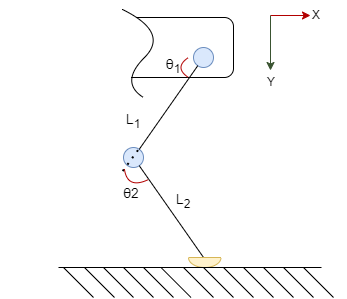
\includegraphics[width=0.5\textwidth]{Areaconfig}
		\caption{Кинематическая схема для определения рабочей области ноги}
		\label{Areaconfig}
	\end{center}
\end{figure}

Используя данные уравнения, которые описывают положение т.B относительно корпуса, а также используя информацию об ограничениях на углы поворота двигателя из таблицы \ref{tablParam}, определим рабочую область ноги (рисунок \ref{workArea}). Алгоритм получения описан в математическом пакете Wolfram Mathematica (Приложение 1). %FIX приложение
\newpage
\begin{figure}[h!]
	\begin{center}
		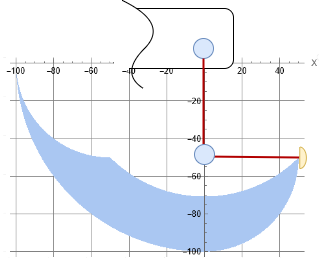
\includegraphics[width=0.8\textwidth]{workArea}
		\caption{Рабочая область ноги робота относительно корпуса}
		\label{workArea}
	\end{center}
\end{figure}


	\newpage
	
\begin{center}
	\textbf{\large ГЛАВА 3 \\ РЕШЕНИЕ ОБРАТНОЙ ЗАДАЧИ КИНЕМАТИКИ}
\end{center}
\refstepcounter{chapter}


% \section*{}
\addcontentsline{toc}{chapter}{ГЛАВА 3}
\section{Общие требования к физической модели четырехногого робота}\label{C4_1}

Все четвероногие животные при движении сохраняют равновесие почти исключительно за счет динамической устойчивости. Изначально план чередования опорных и свободных положений ног заключался в переключении фаз по принципу ноги 1-4 опорная фаза, ноги 2-3 свободная, как показано на рисунке \ref{cycle_wanted}. Зелеными стрелками обозначены фазы свободного положения, а красными опорного. Однако, такой подход не совсем точен, хоть и вполне логичен.
\begin{figure}[h!]
	\begin{center}
		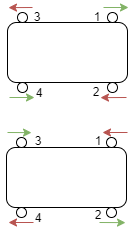
\includegraphics[width=0.3\textwidth]{cycle_wanted}
		\caption{Смена опорных и свободных фаз.}
		\label{cycle_wanted}
	\end{center}
\end{figure}

В случае искусственных шагающих аппаратов походка должны быть определена таким образом, чтобы центр тяжести аппарата постоянно находился внутри треугольника, вершинами которого являются конечности, находящиеся на данный момент времени в опорном положении (рисунок \ref{diagrama}). На практике эта возможность была реализована д-ром Такути из Научно-исследовательского центра проблем механики\cite{Nakano}. Под его руководством был разработан шагающий аппарат с четырьмя конечностями, у которых скорость движения в фазе восстановления подобрана так, что длительность этой фазы втрое меньше длительности каждой рабочей фазы. В результате в данный момент времени лишь одна нога робота находится в воздухе, а корпус опирается на три остальные, сохраняя тем самым статическую устойчивость. 

Показанные на рисунке заштрихованные треугольники (так называемые опорные треугольники) образованы вершинами, которые соответствуют текущим точкам касания опорной поверхности какими-либо тремя из четырех ног робота. Например, в состоянии, соответствующем рисунку \ref{diagrama}, опоры касаются три ноги - А, В, С, а четвертая нога - D, будучи в фазе восстановления, находится в воздухе. Для обеспечения статической устойчивости принципиально важное значение имеет правильный выбор порядка чередования (сдвиг фаз) четырех ног в процессе движения аппарата. В момент времени, отраженный на диаграмме 1, нога В только что коснулась земли и сейчас занимает опорное положение, нога А также касается земли, но находится уже во второй половине своей рабочей фазы, а нога С - еще в первой половине собственной рабочей фазы. Нога D, находящаяся в момент наблюдения в воздухе, быстро заканчивает фазу восстановления, и к моменту времени, которому соответствует диаграмма 2, она уже опускается на землю, переходя в опорное положение. К этому моменту нога А завершила свою рабочую фазу и, оторвавшись от земли, переходит в фазу восстановления; нога В находится в первой половине, а нога С - во второй половине своих рабочих фаз. Аналогично в следующие моменты времени, которым соответствуют диаграммы 3 и 4, в фазу восстановления переходят друг за другом нога С и нога В. 

При таком порядке чередования ног в любой момент времени, когда одна из ног робота находится в фазе восстановления, центр тяжести аппарата обязательно будет лежать внутри треугольника, образованного тремя ногами, находящимися не в рабочей фазе (опирающимися на землю).

\begin{figure}[h!]
	\begin{center}
		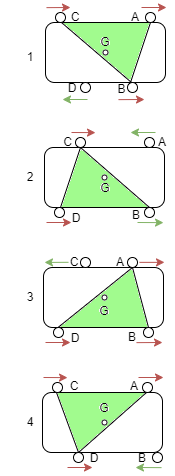
\includegraphics[width=0.3\textwidth]{diagrama}
		\caption{Смена опорных и свободных фаз с учетом тяжести}
		\label{diagrama}
	\end{center}
\end{figure}
\newpage
\section{Задача синтеза походки четырехногого шагающего робота}\label{C3_1}
Процесс движения шагающего аппарата, в котором осуществляется работа ног, можно определить как ходьбу. В ходе данного процесса каждая из ног может находиться в одном из двух основных состояний, отличающихся друг от друга принципиально.

В процессе ходьбы, ноги шагающего аппарата попеременно занимают то опорное, то свободное положения, причем в течение одного цикла каждая нога занимает то и другое положение один раз. Последовательность, в которой при ходьбе происходит чередование опорного и свободного положений всех ног аппарата, определяет конкретный способ его передвижения или его походку. Последовательность чередований ног за один период называется циклом ходьбы, а расстояние, которое проходит аппарат за один цикл, - шагом\cite{Nakano}.
Движения, совершаемые любой из ног при чередовании опорного и свободного положений в процессе ходьбы, можно упрощенно разделить на фазу поступательного перемещения и фазу восстановления. В простейшем случае переход от первой фазы ко второй может осуществляться за счет движений ноги вверх-вниз строго по вертикали. Однако энергия шагающего аппарата будет расходоваться более эффективно, если в течение фазы восстановления нога будет перемещаться по некоторой кривой. Одна из возможных форм криволинейной траектории стопы относительно корпуса показана на рис \ref{movement}. 

Разделим предстоящую задачу формирования походки на два этапа:

\begin{enumerate} 
	\item Опорное положение (перенос корпуса) - в это время нога касается поверхности и служит опорной для корпуса аппарата;
	\item Свободное положение (перенос ноги) - в это время нога находится над поверхностью и готовится к выполнению опорных функций на следующем шаге.
\end{enumerate}
\newpage
\begin{figure}[h!]
	\begin{center}
		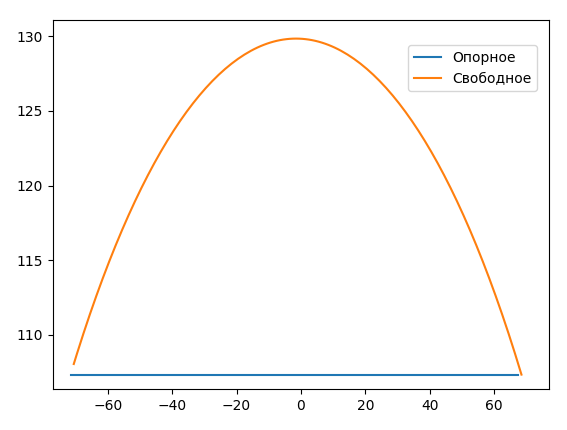
\includegraphics[width=0.8\textwidth]{movement}
		\caption{Фазы опорного и свободного положения ноги во время движения}
		\label{movement}
	\end{center}
\end{figure}

\section{Решение задачи для одной ноги. Опорное положение}\label{C3_2}
Рассмотрим подробно первый этап. Нам известны длины звеньев $L_{1}$ и $L_{2}$, а также высота от поверхности земли до корпуса $h_{\text{корп}}$. 
Начальные условия для шага:
\begin{equation}
	\begin{array}{l}
		X = +X_{\text{ш}},
		\\
		Y = 0.
	\end{array}
\end{equation}
Конечные условия для шага:
\begin{equation}
	\begin{array}{l}
		X = -X_{\text{ш}},
		\\
		Y = 0,
	\end{array}
	\label{gran_step}
\end{equation}
где $X_{\text{ш}}$ - максимальное значение для переноса корпуса во время опорной фазы, -$X_{\text{ш}}$ - максимальное значение для переноса ноги во время свободной фазы. Отрезок от -$X_{\text{ш}}$ до $X_{\text{ш}}$ - полная ширина шага.  

Таким образом, положение ноги в начальный момент времени можно отобразить согласно рисунку \ref{Plus_step}.
\newline
\begin{figure}[h]
	\begin{center}
		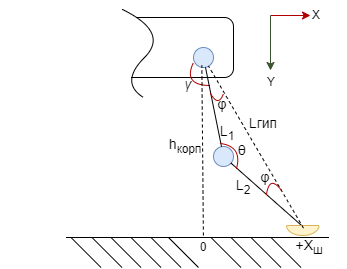
\includegraphics[width=0.6\textwidth]{Plus_step}
		\caption{Положения ноги относительно корпуса в начальный момент времени}
		\label{Plus_step}
	\end{center}
\end{figure}

В данной задаче необходимо определить закон изменения углов двигателей в бедре $\gamma$ и колене $\theta$ для положительного переноса корпуса по оси $X$. Исходя из рисунка \ref{Plus_step}, получим следующие уравнения для $\gamma$:
\begin{equation}
	\begin{array}{l}
		\phi+\gamma-\displaystyle\frac{\pi}{2} = \arcctg\left({\displaystyle\frac{+X_{\text{ш}}}{h_{\text{корп}}}}\right), 
		\\
		\gamma = \displaystyle\frac{\pi}{2}+ \arcctg\left({\displaystyle\frac{+X_{\text{ш}}}{h_{\text{корп}}}}\right) - \Phi.
	\end{array}
\end{equation}
Соответственно для $\theta$ получим:
\begin{equation}
	\begin{array}{l}
		\theta = 2 \arcsin\left({\displaystyle\frac{l_{\text{гип}}}{2l_{1}}}\right),	
	\end{array}			
\end{equation}
где вспомогательный угол $\phi$ и длину $l_{\text{гип}}$ можно найти как:
\begin{equation}
	\begin{array}{l}
		\phi=\arccos\left({\displaystyle\frac{l_{\text{гип}}}{2l_{1}}}\right),
		\\
		l_{\text{гип}}=\sqrt{x^{2}_{\text{ш}}+h^{2}_{\text{корп}}}.
	\end{array}
\end{equation}

Далее рассмотрим конечный момент времени, где условия шага описаны формулой \ref{gran_step}. Конфигурация ноги в таком случае примет положение, которое отображено на рисунке \ref{minus_step}.
\begin{figure}[h!]
	\begin{center}
		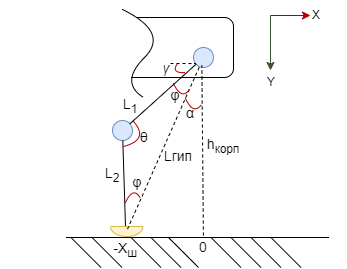
\includegraphics[width=0.6\textwidth]{minus_step}
		\caption{Положения ноги относительно корпуса в конечный момент времени}
		\label{minus_step}
	\end{center}
\end{figure}

Определим значения, которые принимают $\gamma$, $\theta$ и вспомогательный угол $\alpha$ в конечный момент времени переноса корпуса.
\begin{equation}
	\begin{array}{l}
		\gamma= \displaystyle\frac{\pi}{2} - \phi - \arctg\left({\displaystyle\frac{-X_{\text{ш}}}{h_{\text{корп}}}}\right) =
		\\
		=\displaystyle\frac{\pi}{2}-\arccos\left({\displaystyle\frac{l_{\text{гип}}}{2l_{1}}}\right)+\arctg\left({\displaystyle\frac{-X_{\text{ш}}}{h_{\text{корп}}}}\right),
		\\
		\theta = 2 \arcsin\left({\displaystyle\frac{l_{\text{гип}}}{2l_{1}}}\right),
		\\
		\alpha = \arctg\left({\displaystyle\frac{-X_{\text{ш}}}{h_{\text{корп}}}}\right).
	\end{array}
\end{equation}

Заметим, что законы изменения углов двигателей отличаются только знаком $X_{\text{ш}}$. Таким образом, определим общий закон изменения углов в зависимости от $X_{\text{ш}}$. Иначе говоря получим решение обратной задачи кинематики для одного шага робота, но без переноса стопы:
\begin{equation}
	\begin{array}{l}
		\theta(x_{\text{ш}}) = 2 \arcsin\left({\displaystyle\frac{\sqrt{x^{2}_{\text{ш}}+h^{2}_{\text{корп}}}}{2l_{1}}}\right),
		\\
		\gamma(x_{\text{ш}})= \displaystyle\frac{\pi}{2} -\arccos\left({\frac{\sqrt{x^{2}_{\text{ш}}+h^{2}_{\text{корп}}}}{2l_{1}}}\right) + \arctg\left({\displaystyle\frac{X_{\text{ш}}}{h_{\text{корп}}}}\right),
		\\
		l_{\text{гип}}=\sqrt{x^{2}_{\text{ш}}+h^{2}_{\text{корп}}}.
	\end{array}
	\label{finalEQ}
\end{equation}

Напишем небольшой скрипт на языке Python, чтобы построить графики изменения углов в двигателях в зависимости от ширины шага $X_{\text{ш}}$:
%\newpage
\begin{python}
	
 	def callculate_step(x_range_step,height):
	
		y_step=0
		height_slew = np.sqrt(x_range_step**2+(height-y_step)**2)
		hip_step = 0.5*np.pi - np.arccos(height_slew/(2*.l1))+np.arctan(x_range_step/(height-y_step))
		knee_step = 2*np.arcsin(height_slew/(2*.l1))
	
	return np.rad2deg(hip_step), np.rad2deg(knee_step)
\end{python}

Получим следующие результаты для значений $X_{\text{ш}}$ от -40 мм до 40 мм с шагом 1 мм. Отобразим их на рисунке \ref{ideal_kin}. Для этого вызовем функцию в исполнительном файле: 
\newpage

\begin{python}
	import numpy as np
	import matplotlib.pyplot as plt
	
	x_range_step = np.arange(40,-40,-10)
	hip_step = np.zeros(np.size(x_range_step))
	knee_step = np.zeros(np.size(x_range_step))

	for i in range(x_range_step):
		hip,knee = callculate_step(x_range_step[i])
		hip_step[i] = hip
		knee_step[i] = knee
	
	plt.plot(hip_step)
	plt.plot(knee_step)
	
\end{python}

\begin{figure}[h!]
	\begin{center}
		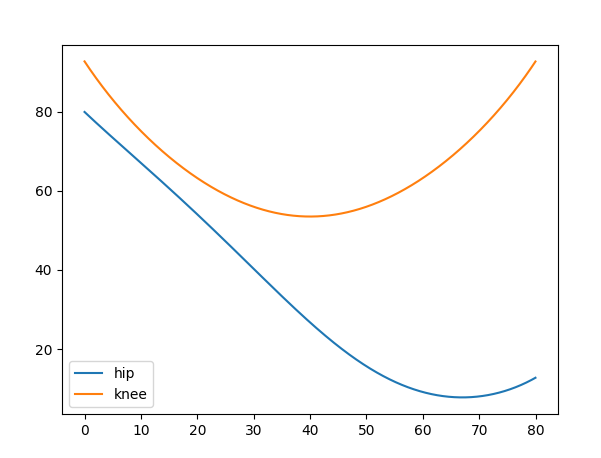
\includegraphics[width=0.9\textwidth]{ideal_kin}
		\caption{График изменения углов бедра и колена во времени}
		\label{ideal_kin}
	\end{center}
\end{figure}

\newpage 
Проверим, что в момент фазы опорного положения ноги, ее высота не изменялась и задача о положении ноги для переноса корпуса решена верно. Если задача решена верно, то результатом уравнения \ref{h_step}, при построении графика должна быть горизонтальная прямая (рисунок \ref{H} ), по значению равная $h_{\text{корп}}$, которая означает, что крайняя точка ноги (стопа) находилась на максимальном заданном расстоянии от корпуса и не изменялась в течение фазы опорного положения:
\begin{equation}
	\begin{array}{l}
		H = l_{1}\cos({\frac{\pi}{2}-\gamma}) + l_{2}\sin({\theta-\gamma}).
	\end{array}
	\label{h_step}
\end{equation}
\newline
\begin{figure}[h!]
	\begin{center}
		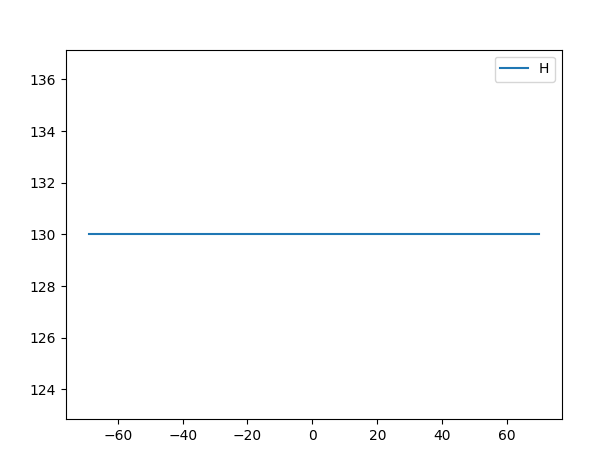
\includegraphics[width=0.9\textwidth]{H}
		\caption{График высоты стопы при опорном положении}
		\label{H}
	\end{center}
\end{figure}
\newpage
\section{Решение задачи для одной ноги. Свободное положение}\label{C3_3}
Фаза переноса - это один из ключевых этапов движения четырехногого робота, который происходит между фазами опоры. Во время переноса конечность робота находятся в воздухе и перемещается в новую позицию для следующего шага. Эта фаза требует от робота сбалансированности и точности движений, чтобы избежать падений и обеспечить плавность передвижения. Иначе говоря, фазу переноса можно рассматривать как переходный этап между двумя фазами опоры, в котором робот готовится к следующему шагу.

Рассмотрим подробно второй этап. Нам известны длины звеньев $L_{1}$, $L_{2}$ и высота от поверхности земли до корпуса $h_{\text{корп}}$. 
Условия для свободного положения включают в себя два краевых: начальное и конечное, а также серединное.
\newline
Начальные условия:
\begin{equation}
	\begin{array}{l}
		X = -X_{\text{ш}},
		\\
		Y = 0.
	\label{gran_skip1}
	\end{array}
\end{equation}
Конечные условия:
\begin{equation}
	\begin{array}{l}
		X = +X_{\text{ш}},
		\\
		Y = 0.
	\label{gran_skip2}
	\end{array}
\end{equation}
Серединные условия:
\begin{equation}
	\begin{array}{l}
		X = 0,
		\\
		Y = h_{\text{под}},
	\end{array}
	\label{gran_skip3}
\end{equation}
где $X_{\text{ш}}$ - максимальное значение для переноса корпуса во время опорной фазы, -$X_{\text{ш}}$ - максимальное значение для переноса ноги во время свободной фазы. Отрезок от -$X_{\text{ш}}$ до $X_{\text{ш}}$ - полная ширина шага. $h_{\text{под}}$ - высота подъема ноги, ограничения на которую необходимо найти.

Рассмотрим кинематическую схему на рисунке \ref{skip_traj}. На нем изображена конфигурация ноги в трех положениях, которые описывают условия \ref{gran_skip1},\ref{gran_skip2},\ref{gran_skip3}. 
\newpage
\begin{figure}[h!]
	\begin{center}
		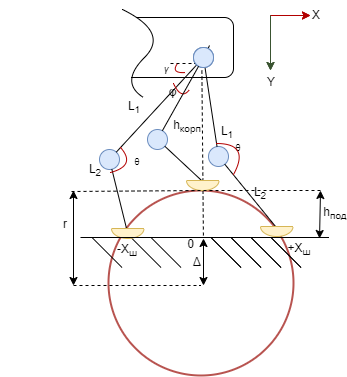
\includegraphics[width=0.6\textwidth]{skip_traj}
		\caption{Последовательность переноса стопы в свободном положении}
		\label{skip_traj}
	\end{center}
\end{figure}

Перенос стопы по дуге окружности не является оптимальным решением, так как при движении по неровной поверхности этот параметр должен изменяться в зависимости от условий. В настоящее время поиск таких траекторий переноса выполняется с опорой на машинное обучение с подкреплением, что требует отдельного исследования. В настоящей работе движение происходит на ровной поверхности, таким образом с помощью регулирования радиуса $r$ создадим механизм, позволяющий регулировать высоту переноса стопы $h_{\text{под}}$, которая будет реализуема для заданной конфигурации робота, с учетом известных длин звеньев $l_{1}$, $l_{2}$ и высоты $h_{\text{корп}}$. Исходя из известных данных, вполне справедливо, что радиус можно найти как:
\begin{equation}
	\begin{array}{l}
		r=\sqrt{x^{2}_{\text{ш}}+\Delta^{2}} = \Delta + h_{\text{под}},
	\end{array}
	\label{radius}
\end{equation}
где $x_{\text{ш}}$ - задаваемая ширина шага от -$X_{\text{ш}}$ до $+X_{\text{ш}}$, $\Delta$ - расстояние, которым контролируется положение центра окружности по высоте.
\newline
Таким образом высота подъема стопы $h_{\text{под}}$ определяется из уравнения:
 \begin{equation}
 	\begin{array}{l}
 		h_{\text{под}}(x_{\text{ш}})=\sqrt{r^{2}-x^{2}_{\text{ш}}}-\Delta,
 		\\
 		\Delta = \sqrt{r^{2}-x^{2}_{\text{ш}}},
 	\end{array}
 	\label{hpod}
 \end{equation}
 где ограничение на высоту подъема ноги вводится как:
 \noindent $$r>x_{\text{ш}}$$
 
 Тогда с учетом найденного $h_{\text{под}}$, определим законы изменения углов в двигателях для бедра и колена соответственно:
 
 \begin{equation}
 	\begin{array}{l}
 		\theta(x_{\text{ш}}) = 2 \arcsin\left({\displaystyle\frac{\sqrt{x^{2}_{\text{ш}}+h^{2}_{\text{корп}}-h^{2}_{\text{под}}}}{2l_{1}}}\right),
 		\\
 		\gamma(x_{\text{ш}})= \displaystyle\frac{\pi}{2} -\arccos\left({\frac{\sqrt{x^{2}_{\text{ш}}+h^{2}_{\text{корп}}-h^{2}_{\text{под}}}}{2l_{1}}}\right) + \arctg\left({\frac{X_{\text{ш}}}{h_{\text{корп}}}}\right),
 		\\
 		l_{\text{гип}}=\sqrt{x^{2}_{\text{ш}}+h^{2}_{\text{корп}}},
 		\\
 		h_{\text{под}}(x_{\text{ш}})=\sqrt{r^{2}-x^{2}_{\text{ш}}}-\Delta,
 		\\
 		\Delta = \sqrt{r^{2}-x^{2}_{\text{ш}}}.
 	\end{array}
 	\label{skip_eq}
 \end{equation}
 
Аналогично с пунктом \ref{C3_2} напишем скрипт на языке Python, чтобы получить графики изменения углов в двигателях в зависимости от ширины шага $X_{\text{ш}}$:

 \begin{python}
	def callculate_skip(x_range_skip,min_delta,height,r):
		delta = np.sqrt(r**2-min_delta**2)
		y_skip = np.sqrt((r**2) - (x_range_skip**2)) - delta
		height_slew = np.sqrt(x_range_skip**2+(height-y_skip)**2)
		
		hip_skip = 0.5*np.pi - np.arccos(height_slew/(2*l1))+np.arctan(x_range_skip/(height-y_skip))
		knee_skip = 2*np.arcsin(height_slew/(2*l1))
		
		return np.rad2deg(hip_skip),np.rad2deg(knee_skip)
\end{python}

C учетом результатов на рисунке \ref{ideal_kin}, получим графики углов $\theta$ и $\gamma$ при переносе стопы для значений $X_{\text{ш}}$ от -40 мм до 40 мм с шагом 1 мм, высотой $h_\text{корп}$ = 130 мм и $r$ = 100 мм. Отобразим их на рисунке \ref{full_traj}. Для этого добавим функцию в исполнительный файл, описанный выше в пункте \ref{C3_2}:

\begin{python}
	import numpy as np
	import matplotlib.pyplot as plt
	
	x_range_step = np.arange(40,-40,-10)
	x_range_skip = np.arange(-40,40,10)
	r= 100
	height = 130
	min_delta = x_range_skip[0]
	hip = []
	knee = []
	
	for i in range(x_range_step):
		hip,knee = callculate_step(x_range_step[i],height)
		hip[i] = hip
		knee[i] = knee
	
	for i in range(x_range_skip):
		hip,knee = callculate_skip(x_range_skip,min_delta,height,r)
		hip[i] = hip
		knee[i] = knee
	
	plt.plot(hip)
	plt.plot(knee)
\end{python}

\begin{figure}[h!]
	\begin{center}
		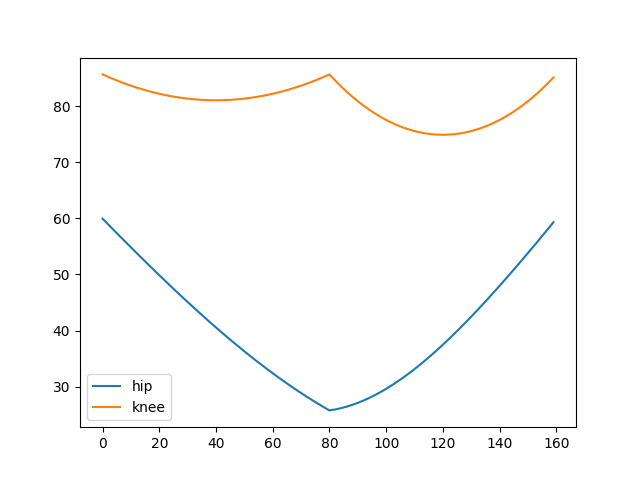
\includegraphics[width=0.8\textwidth]{full_traj}
		\caption{Изменение углов двигателей за полный цикл одного шага}
		\label{full_traj}
	\end{center}
\end{figure}
%\noindent
%\newpage
Проведем проверку, аналогичную в пункте \ref{C2_2}. Если задача решена верно, то мы получим результат схожий с рисунком \ref{movement}. Для этого воспользуемся формулой \ref{h_step}. Полученный график отображен на рисунке \ref{full_cycle}
\newpage
\begin{figure}[h!]
	\begin{center}
		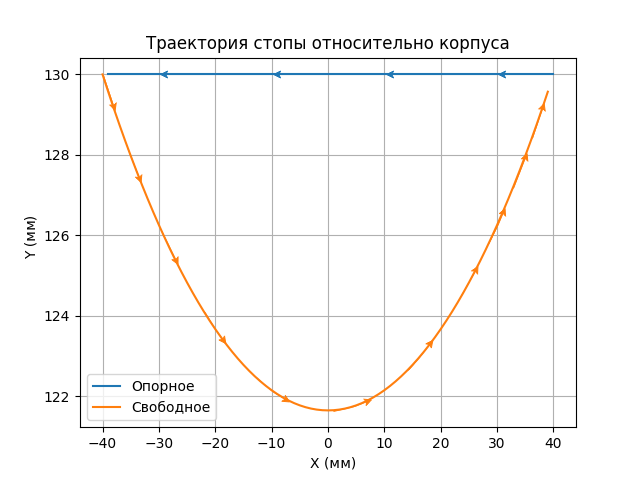
\includegraphics[width=0.7\textwidth]{full_cycle}
		\caption{Траектория стопы относительно корпуса за полный шаг}
		\label{full_cycle}
	\end{center}
\end{figure}

\newpage
	\newpage
	\newpage
\begin{center}
	\textbf{\large ГЛАВА 4 \\ МОДЕЛИРОВАНИЕ И СБОРКА}
\end{center}
\refstepcounter{chapter}


% \section*{}
\addcontentsline{toc}{chapter}{ГЛАВА 4}
%\section{Общие требования к физической модели четырехногого робота}\label{C4_1}

%Все четвероногие животные при движении сохраняют равновесие почти исключительно за счет динамической устойчивости. Изначально план чередования опорных и свободных положений ног заключался в переключении фаз по принципу ноги 1-4 опорная фаза, ноги 2-3 свободная, как показано на рисунке \ref{cycle_wanted}. Зелеными стрелками обозначены фазы свободного положения, а красными опорного. Однако, такой подход не совсем точен, хоть и вполне логичен.
%\begin{figure}[h!]
%	\begin{center}
%		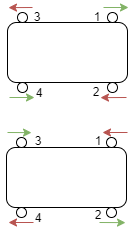
\includegraphics[width=0.3\textwidth]{cycle_wanted}
%		\caption{Смена опорных и свободных фаз.}
%		\label{cycle_wanted}
%	\end{center}
%\end{figure}

%  В случае искусственных шагающих аппаратов походка должны быть определена таким образом, чтобы центр тяжести аппарата постоянно находился внутри треугольника, вершинами которого являются конечности, находящиеся на данный момент времени в опорном положении (рисунок \ref{diagrama}). На практике эта возможность была реализована д-ром Такути из Научно-исследовательского центра проблем механики\cite{Nakano}. Под его руководством был разработан шагающий аппарат с четырьмя конечностями, у которых скорость движения в фазе восстановления подобрана так, что длительность этой фазы втрое меньше длительности каждой рабочей фазы. В результате в данный момент времени лишь одна нога робота находится в воздухе, а корпус опирается на три остальные, сохраняя тем самым статическую устойчивость. 
  
%  Показанные на рисунке заштрихованные треугольники (так называемые опорные треугольники) образованы вершинами, которые соответствуют текущим точкам касания опорной поверхности какими-либо тремя из четырех ног робота. Например, в состоянии, соответствующем рисунку \ref{diagrama}, опоры касаются три ноги - А, В, С, а четвертая нога - D, будучи в фазе восстановления, находится в воздухе. Для обеспечения статической устойчивости принципиально важное значение имеет правильный выбор порядка чередования (сдвиг фаз) четырех ног в процессе движения аппарата. В момент времени, отраженный на диаграмме 1, нога В только что коснулась земли и сейчас занимает опорное положение, нога А также касается земли, но находится уже во второй половине своей рабочей фазы, а нога С - еще в первой половине собственной рабочей фазы. Нога D, находящаяся в момент наблюдения в воздухе, быстро заканчивает фазу восстановления, и к моменту времени, которому соответствует диаграмма 2, она уже опускается на землю, переходя в опорное положение. К этому моменту нога А завершила свою рабочую фазу и, оторвавшись от земли, переходит в фазу восстановления; нога В находится в первой половине, а нога С - во второй половине своих рабочих фаз. Аналогично в следующие моменты времени, которым соответствуют диаграммы 3 и 4, в фазу восстановления переходят друг за другом нога С и нога В. 
  
%  При таком порядке чередования ног в любой момент времени, когда одна из ног робота находится в фазе восстановления, центр тяжести аппарата обязательно будет лежать внутри треугольника, образованного тремя ногами, находящимися не в рабочей фазе (опирающимися на землю).
  
%\begin{figure}[h!]
%  	\begin{center}
%  		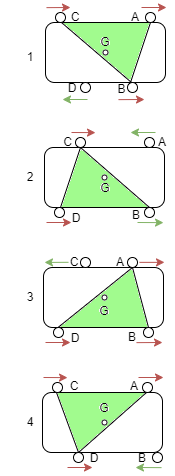
\includegraphics[width=0.3\textwidth]{diagrama}
%  		\caption{Смена опорных и свободных фаз с учетом тяжести}
%  		\label{diagrama}
%  	\end{center}
%\end{figure}

%\newpage

\section{Проектирование ног}\label{C4_2}

В разделе \ref{C1_2} были представлены особенности конструкции и основные проблемы, которые необходимо решить перед производством деталей. 

Для минимизации проблем, связанных с соосностью отверстий, отношениями и масштабами между конструкциями перед этапом печати, были использовали трехмерные твердотельные чертежи при проектировании ног в формате 3D (рисунок \ref{leg_3D}). В качестве материала для изготовления деталей ног был выбран пластик, который используется при печати с помощью 3D-принтера, поскольку уникальная конструкция ног не позволяет использовать доступные металлические изделия для сборки. Кроме того, использование пластика значительно снижает вес конструкции, что позволяет использовать менее мощные двигатели для создания прототипа. Напечатанные и собранные конструкции ног отображены на рисунках \ref{leg2}, \ref{leg3}.
%\newpage  
\begin{figure}[h!]
	\begin{center}
		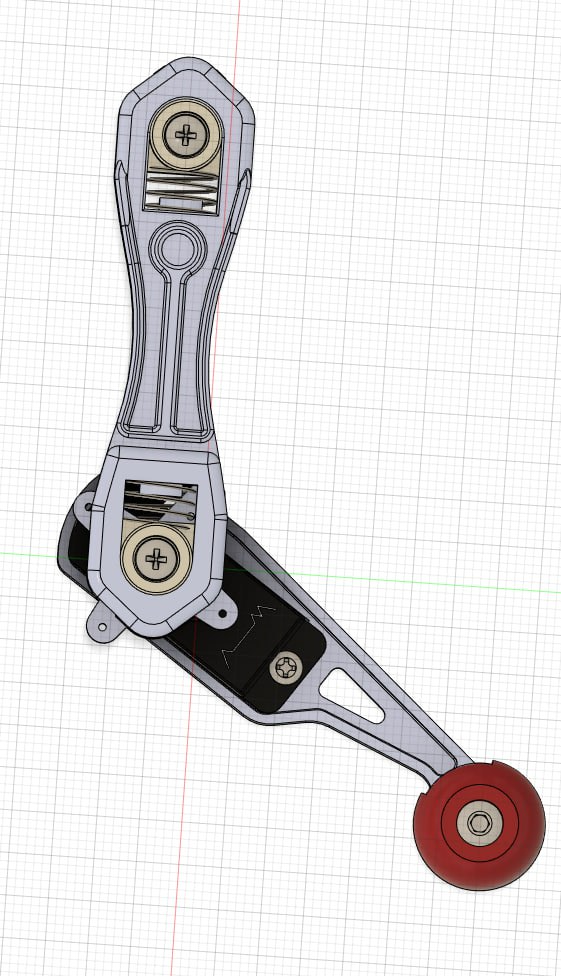
\includegraphics[width=0.35\textwidth]{leg_3D}
		\caption{Твердотельный чертеж ноги робота}
		\label{leg_3D}
	\end{center}
\end{figure}

%\newpage
Сервоприводы, как в сочленении ног, так и в месте соединения с корпусом, закреплены к ползуну, который в свою очередь подпирается пружиной. Ползун обладает "Т" \space образной формой (рисунок \ref{polzun}), которая поддерживает его в плоскости ноги и не дает покинуть область конструкции. 

Пружина служит в качестве демпфера, который гасит ударные воздействия на вал двигателя при движении робота, а также оказывает некоторое полезное сопротивление при резком изменении угла поворота двигателя, что не раз спасало прототип при "живом" \space тестировании походки.

\begin{figure}[h!]
	\begin{center}
		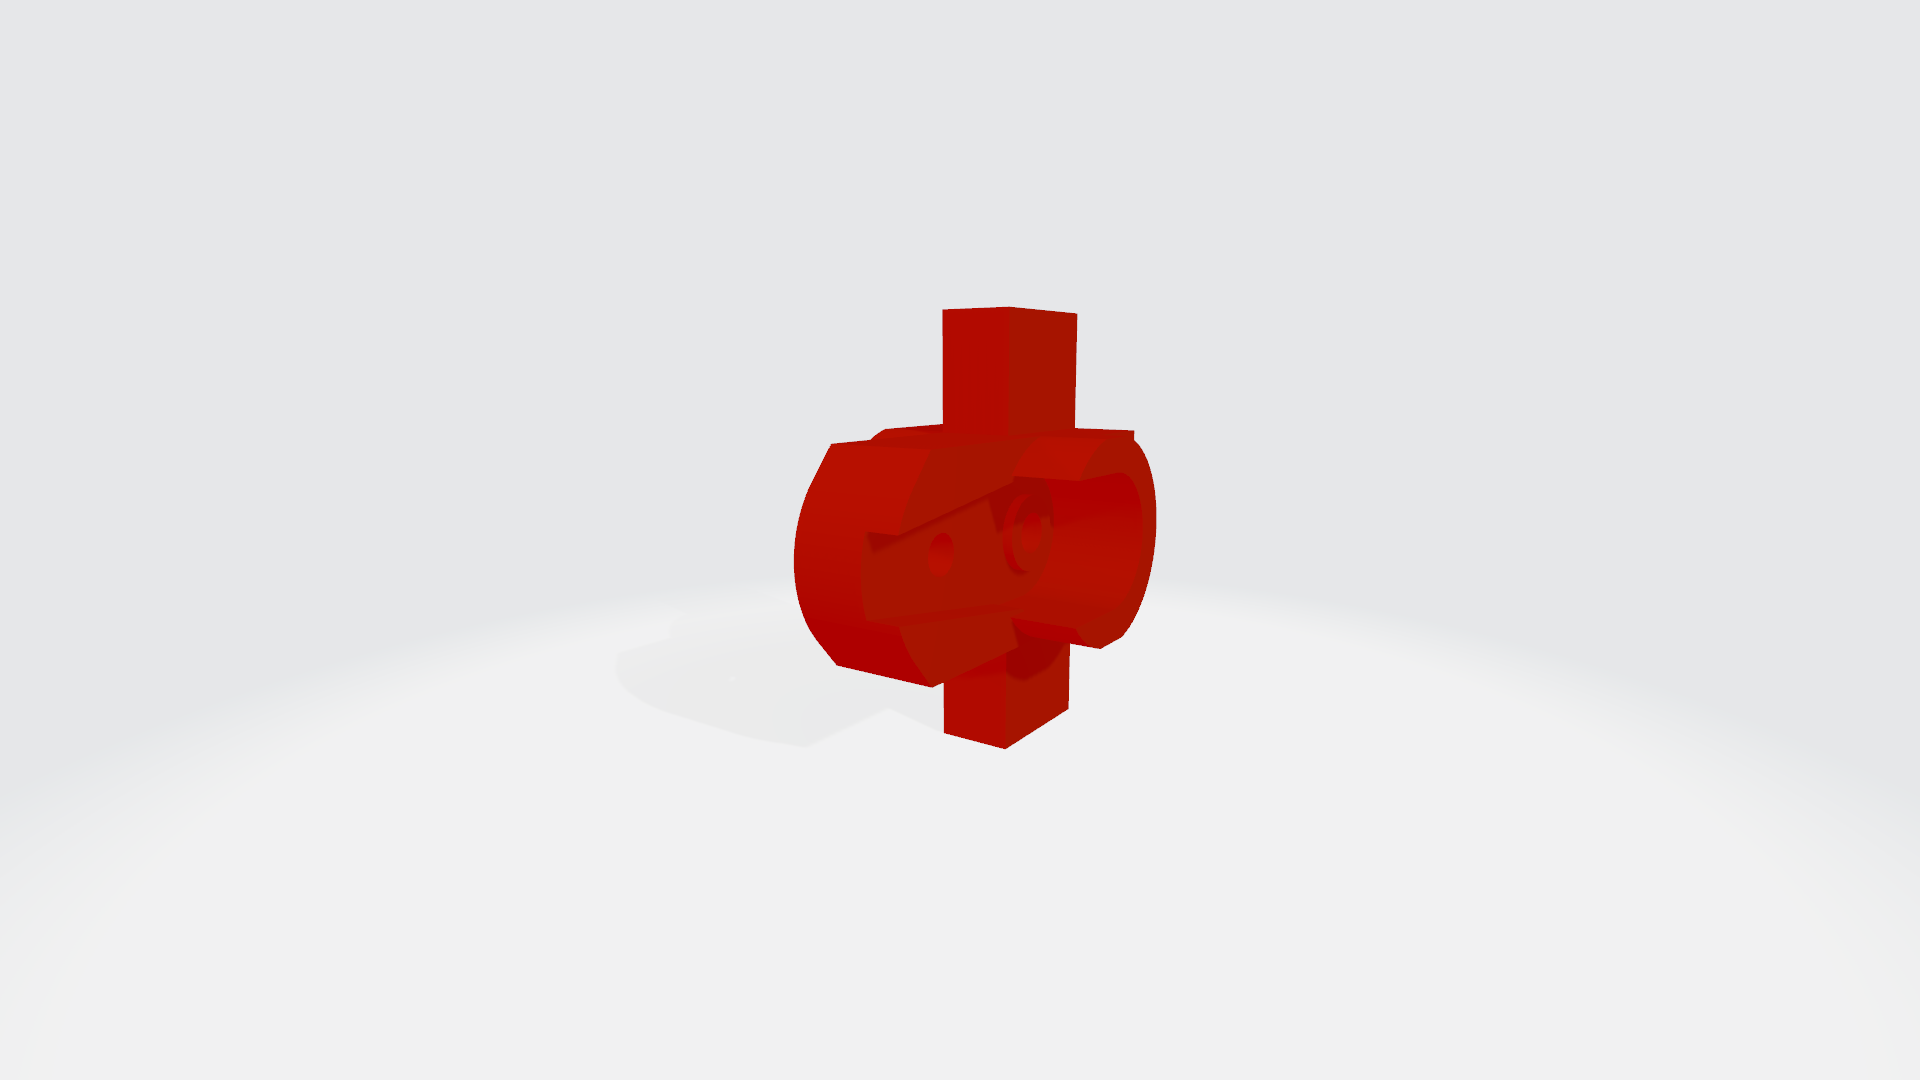
\includegraphics[width=0.8\textwidth]{polzun}
		\caption{\text{''T''} - образный ползун}
		\label{polzun}
	\end{center}
\end{figure}
%\newpage

\begin{figure}[h!]
	\begin{center}
		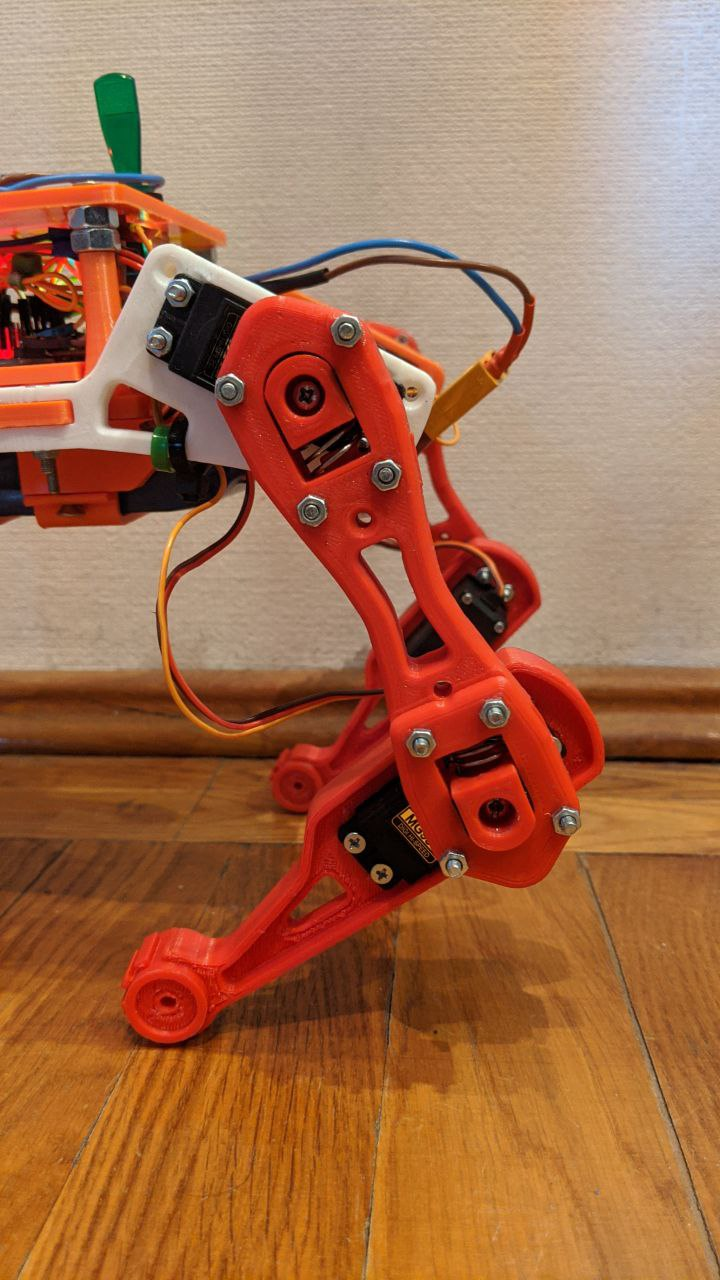
\includegraphics[width=0.4\textwidth]{leg2}
		\caption{Напечатанная нога в сборке}
		\label{leg2}
	\end{center}
\end{figure}

\begin{figure}[h!]
	\begin{center}
		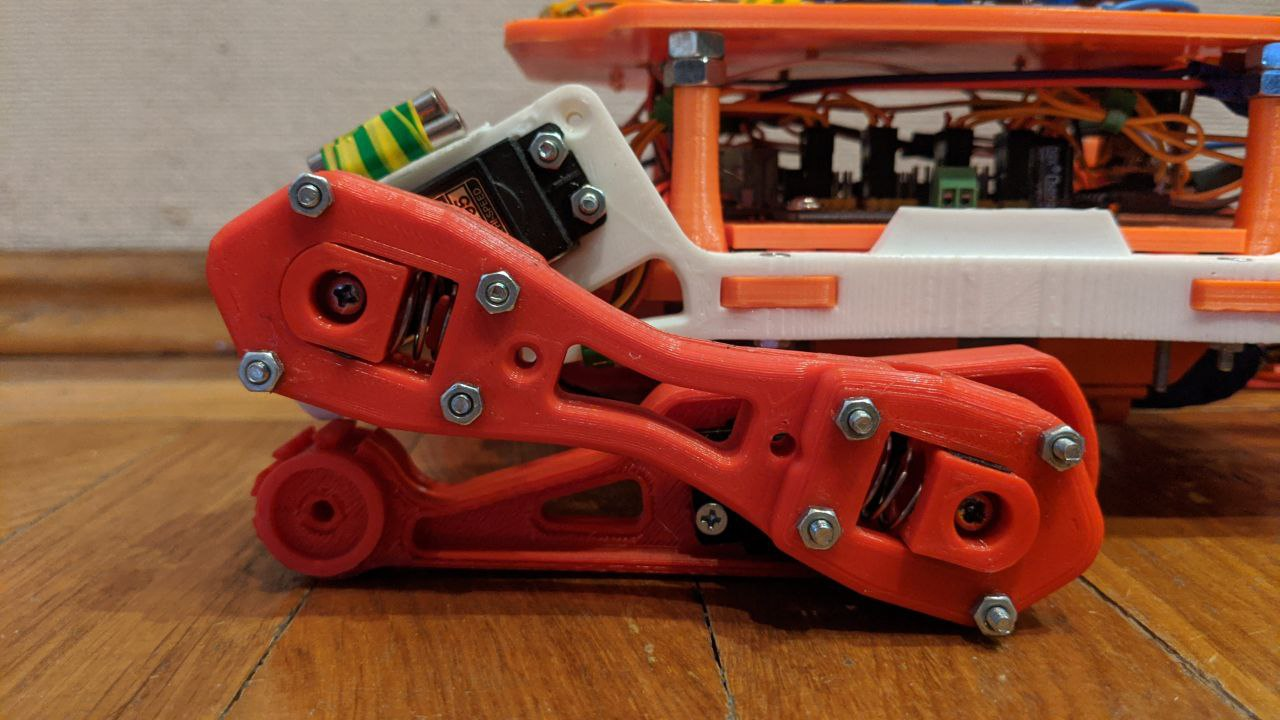
\includegraphics[width=0.5\textwidth]{leg3}
		\caption{Робот в исходном положении до инициализации}
		\label{leg3}
	\end{center}
\end{figure}

\newpage
\section{Проектирование корпуса}\label{C4_3}

Корпус для робота представляет из себя поперечные пластины (рисунок \ref{plastina}), соединенные с лонжеронами. Данные пластины несут функцию размещения электронных компонентов и создания жесткости конструкции. 

\begin{figure}[h!]
	\begin{center}
		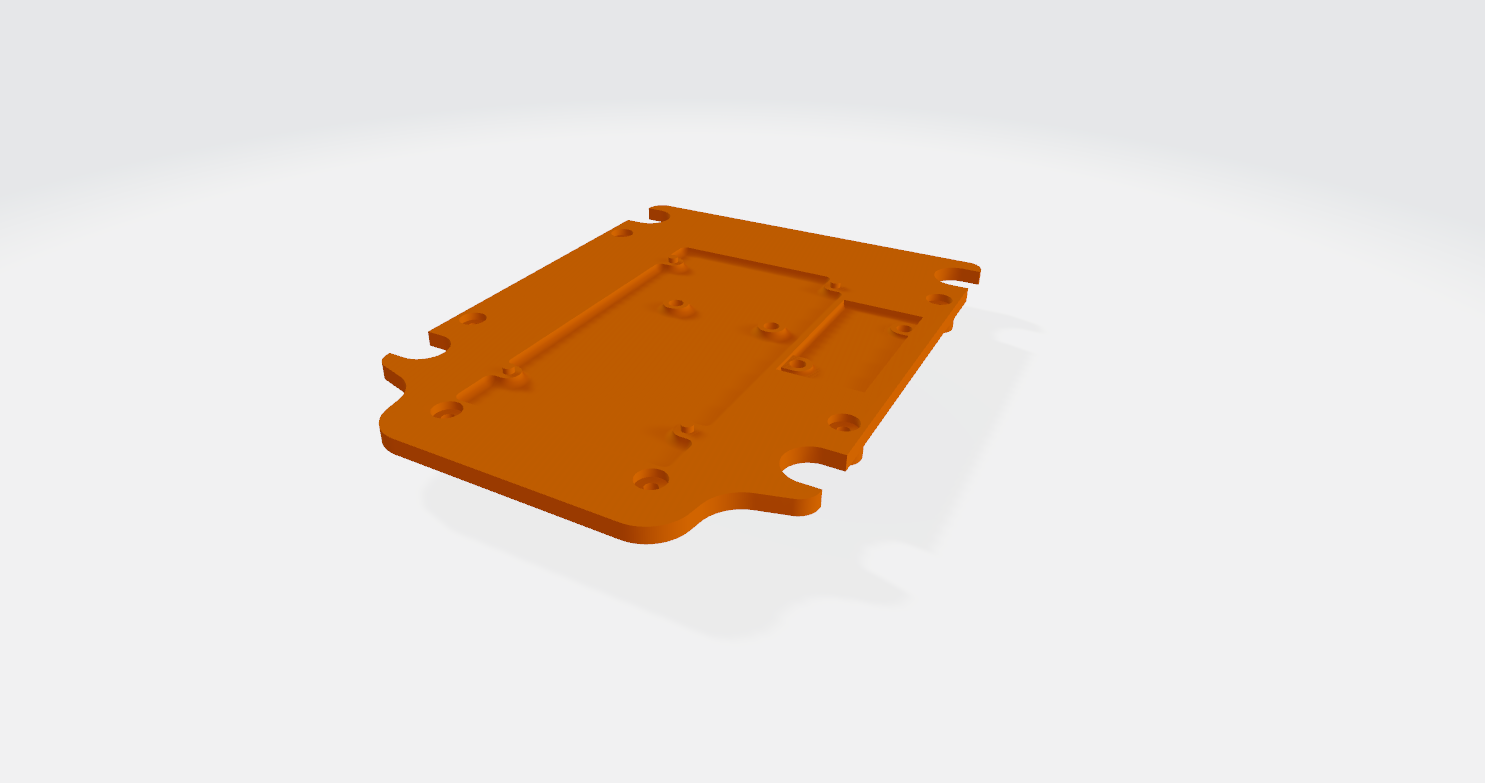
\includegraphics[width=0.8\textwidth]{plastina}
		\caption{Твердотельный чертеж пластины корпуса}
		\label{plastina}
	\end{center}
\end{figure}

В качестве детали к которой крепятся ноги робота, были выбраны лонжероны, также изготовленные из пластика (рисунок \ref{longeron}). Данное решение было принято из-за легкости материала и достаточной жесткости, необходимой для удержания закрепленных деталей. 

\begin{figure}[h!]
	\begin{center}
		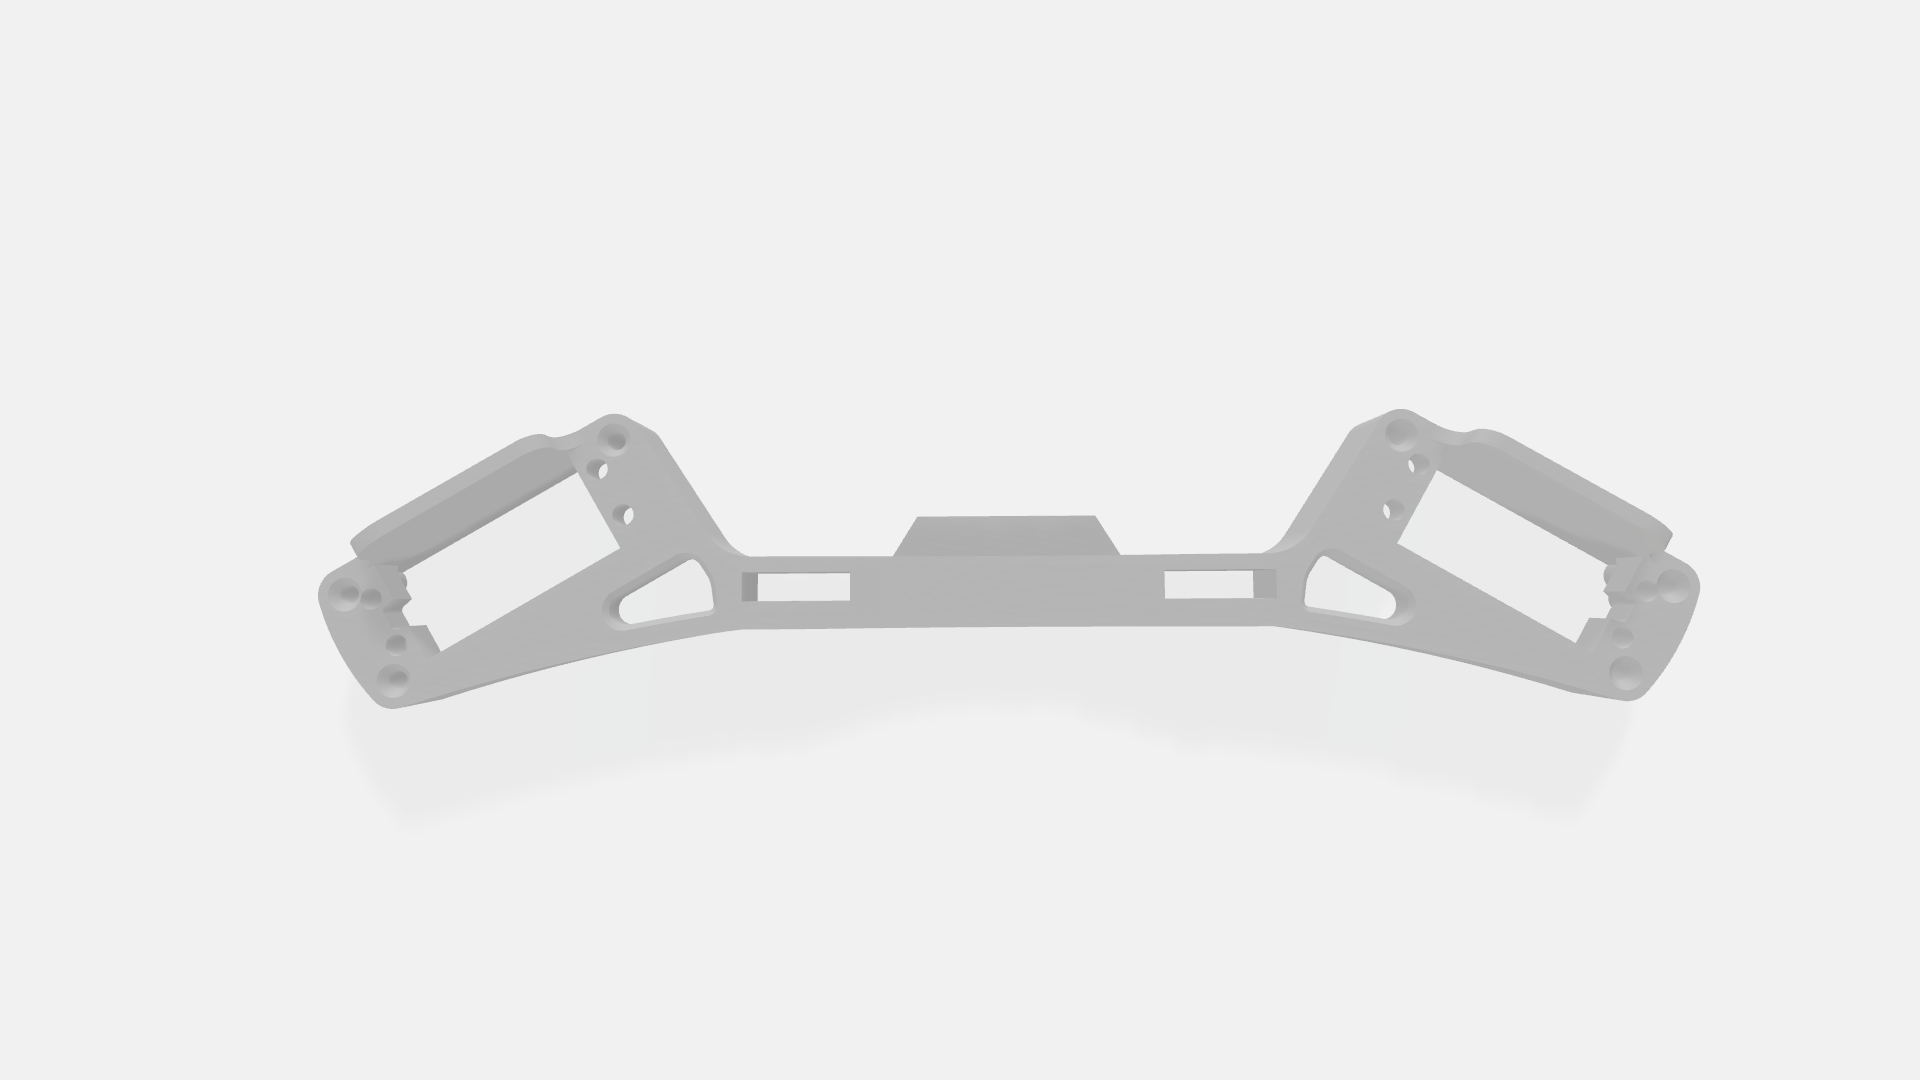
\includegraphics[width=0.8\textwidth]{longeron}
		\caption{Твердотельный чертеж лонжерона корпуса}
		\label{longeron}
	\end{center}
\end{figure}
\pagebreak
В отличие от ног, к корпусу были только минимальные требования, а именно небольшой вес и удобное расположение модулей для последующего подключения. На верхнем уровне корпуса расположены DC/DC преобразователи и трехосевой гироскоп акселерометр MPU6050. На нижнем уровне располагается миникомпьютер OrangePi 3 LTS и ШИМ контроллер PCA9685, в то время как с обратной стороны пластины закреплен источник питания в виде Li-Po аккумулятора (более подробно о подборе комплектующих в разделе \ref{C4_4_1}).


\section{Выбор комплектующих}\label{C4_4}
	\subsection{Выбор сервоприводов}\label{C4_4_1}
	
Сервопривод - это механический привод, который содержит датчик (для измерения положения, скорости, усилия и других параметров) и блок управления приводом (который может быть электронной схемой или механической системой тяг), что позволяет автоматически поддерживать необходимые параметры на датчике в соответствии с заданным внешним значением (например, положение ручки управления или численное значение от других систем). Сервопривод можно рассматривать как автоматического точного исполнителя, который получает на вход значение управляющего параметра в режиме реального времени и используя показания датчика, стремится создать и поддерживать это значение на выходе исполнительного элемента. 

В данной работе предлагается рассчитать максимальный крутящий момент при худшем случае конфигурации робота. При выборе сервопривода данный параметр особенно значим, так как все остальные характеристики вроде габаритов и мест размещения крепежей у этих типов двигателей мало отличаются. Для того чтобы рассчитать худший случай нагрузки и выбрать подходящий сервопривод, необходимо знать следующие параметры:
\begin{itemize}
	\item Общий вес робота;
	\item Длины ног.
\end{itemize}

Худшей конфигурацией является случай, когда все ноги робота вытянуты в "струнку" (рисунок \ref{badass}). В таком случае серводвигателям необходимо приложить максимальный крутящий момент для возврата в рабочую конфигурацию.

\begin{figure}[h!]
	\begin{center}
		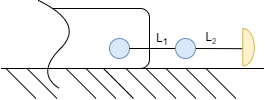
\includegraphics[width=0.5\textwidth]{badass}
		\caption{{Худшая конфигурация для статического случая}}
		\label{badass}
	\end{center}
\end{figure}

Учитывая параметры из таблицы \ref{tablParam}, а также взвесив корпус, с заранее установленными комплектующими, вес робота составляет 1.6 кг. Будем считать, что движения ног для возвращения в исходную конфигурацию будет происходить синхронно, то есть общую нагрузку можно разделить на четыре ноги, что составляет 0.4 кг на одну ногу. Предлагается следующая формула для вычисления максимального момента на одну ногу в случае худшей конфигурации:
 \begin{equation}
	\begin{array}{l}
		M^{\text{крут}}_{\text{макс}} = \displaystyle\frac{m_{\text{роб}}g}{4}(l_{1}+l_{2}).
	\end{array}
	\label{max_moment}
\end{equation}

Исходя из формулы \ref{max_moment} был получен крутящий момент равный 0.8 Нм. В настоящей работе выбрана модель сервопривода MG995, которая полностью удовлетворяет требованиям. Основные характеристики данного привода сведены в таблице \ref{servoParam}.


\begin{table}[h]
	\begin{center}
		\caption{Характеристики сервопривода MG995}
		\label{servoParam}
		\begin{tabular}{| l | l |}
			\hline
			Общий вес   &    55 г \\ \hline
			Размеры (ШхВхГ) & 54х47.2х20 мм\\ \hline
			Крутящий момент & 8.5кгс/см (4.8В), 10кгс/см (6В) \\ \hline
			Рабочая скорость & 0.2с/60$^{\circ}$ (4.8В), 0.16с/60$^{\circ}$ (6В) \\ \hline
			Рабочее напряжение & 4.8В - 7.2В \\ \hline
			Рабочая температура & 0 C$^{\circ}$  - 55 C$^{\circ}$ \\ \hline
			Зона нечувствительности ШИМ & 5мкс \\ \hline
		\end{tabular}
	\end{center}
\end{table} 

Одним из самых главных минусов при работе с сервоприводами является гибкость управления валом двигателя. Резкие изменения угла в серводвигателях являются следствием специфики их конструкции, а если быть точнее, то данная проблема связана с принципом работы потенциометра, который выполняет роль энкодера внутри двигателя. Таким образом принцип регулирования угла поворота состоит в подаче ШИМ сигнала посредством написанного программного обеспечения, сам сигнал преобразуется в напряжение благодаря работе потенциометра и приводит вал в заданное положение с максимальной скоростью. Из этого можно сделать вывод, что в используемых  сервоприводах не имеется обратной связи, и при использовании с тяжелыми объектами будут создаваться лишние нагрузки, которые будут приводить к потреблению тока, особенно это важно по отношению к стартовым токам. В нашем случае такое поведение потенциально приведет к уничтожению редуктора внутри двигателя (рисунок \ref{servo_scheme}), так как движимые объекты инерционные и такое управление для них неприемлемо. Решение этой проблемы подробной разобрано в главе \ref{C5_1}. 

\begin{figure}[h!]
	\begin{center}
		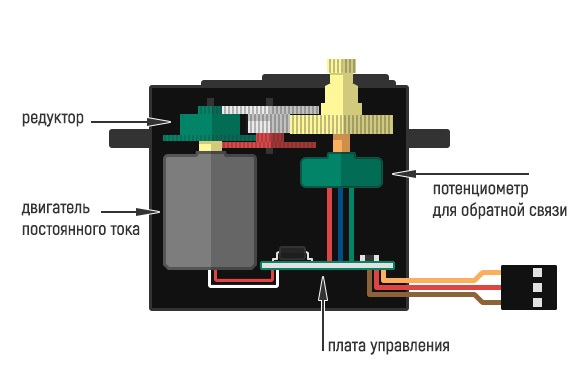
\includegraphics[width=0.7\textwidth]{servo_scheme}
		\caption{Схема сервопривода}
		\label{servo_scheme}
	\end{center}
\end{figure}

Еще одним последствием такого принципа работы выступает осложнение корректной сборки, так как для правильной конфигурации ноги на прототипе сервоприводам требуется калибровка. Иначе говоря, необходимо выставлять крайние положения ног и рассчитывать диапазон ШИМ сигнала и принимаемого угла, чтобы как можно точнее задавать положение ноги в будущем. Это достаточно неприятное следствие, так как каждая единица серводвигателя уникальна и требует отдельной калибровки. Методы калибровки в данной работе разбираться не будут.

\subsection{Выбор управляющей электроники}\label{C4_4_2}
	
В качестве управляющей платы миникомпьютера была выбрана OrangePi 3 LTS (рисунок \ref{orange_pi}). Данный миникомпьютер покрывает все технические требования прототипа сверх нормы, что позволяет не задумываться о методах опрашивания датчиков или скорости обработки информации. Также весомым преимуществом такого компьютера является автономность и наличие встроенной ОС Linux. Такие особенности позволяют использовать плату в привычном для разработчика режиме и не терять время на настройку программного окружения. 	
\begin{figure}[h!]
	\begin{center}
		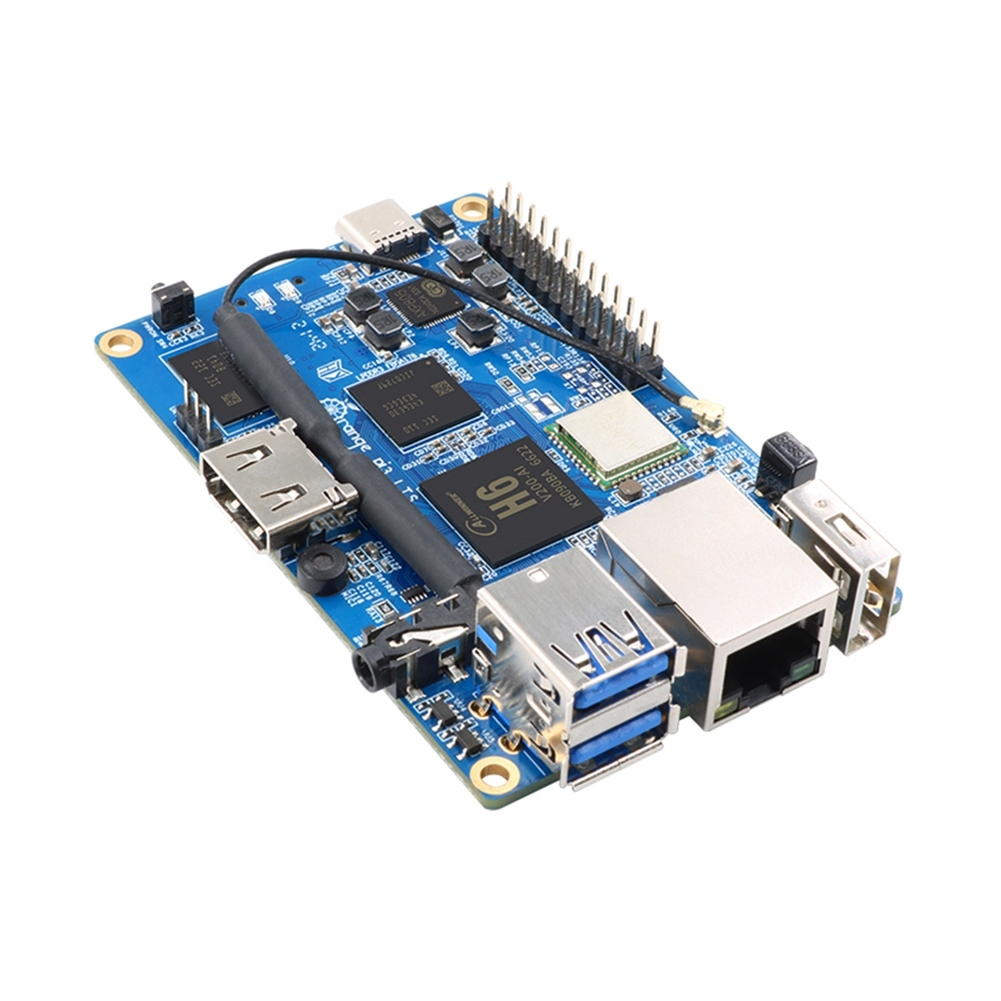
\includegraphics[width=0.4\textwidth]{orange_pi}
		\caption{OrangePi 3 LTS}
		\label{orange_pi}
	\end{center}
\end{figure}

Так как OrangePi не поддерживает управление восемью серводвигателями одновременно, было предложено использовать ШИМ контроллер. В качестве данного контроллера был выбран модуль PCA9685 (рисунок \ref{pca9685}). PCA9685 - это высокопроизводительный драйвер сервоприводов, разработанный фирмой NXP Semiconductors. Он обладает шестнадцатью независимыми каналами широтно-импульсной модуляции (PWM), каждый из которых может управлять сервоприводом. Также PCA9685 имеет встроенную функцию автоматического обновления адресов, что позволяет подключать несколько драйверов к одной шине I2C. Такой подход позволяет назначить уникальный адрес для каждого подключения, чтобы добиться одновременного управления большим количеством сервоприводов. Драйвер также поддерживает частоту ШИМ до 1 кГц, что обеспечивает высокую точность управления сервоприводами.

\begin{figure}[h!]
	\begin{center}
		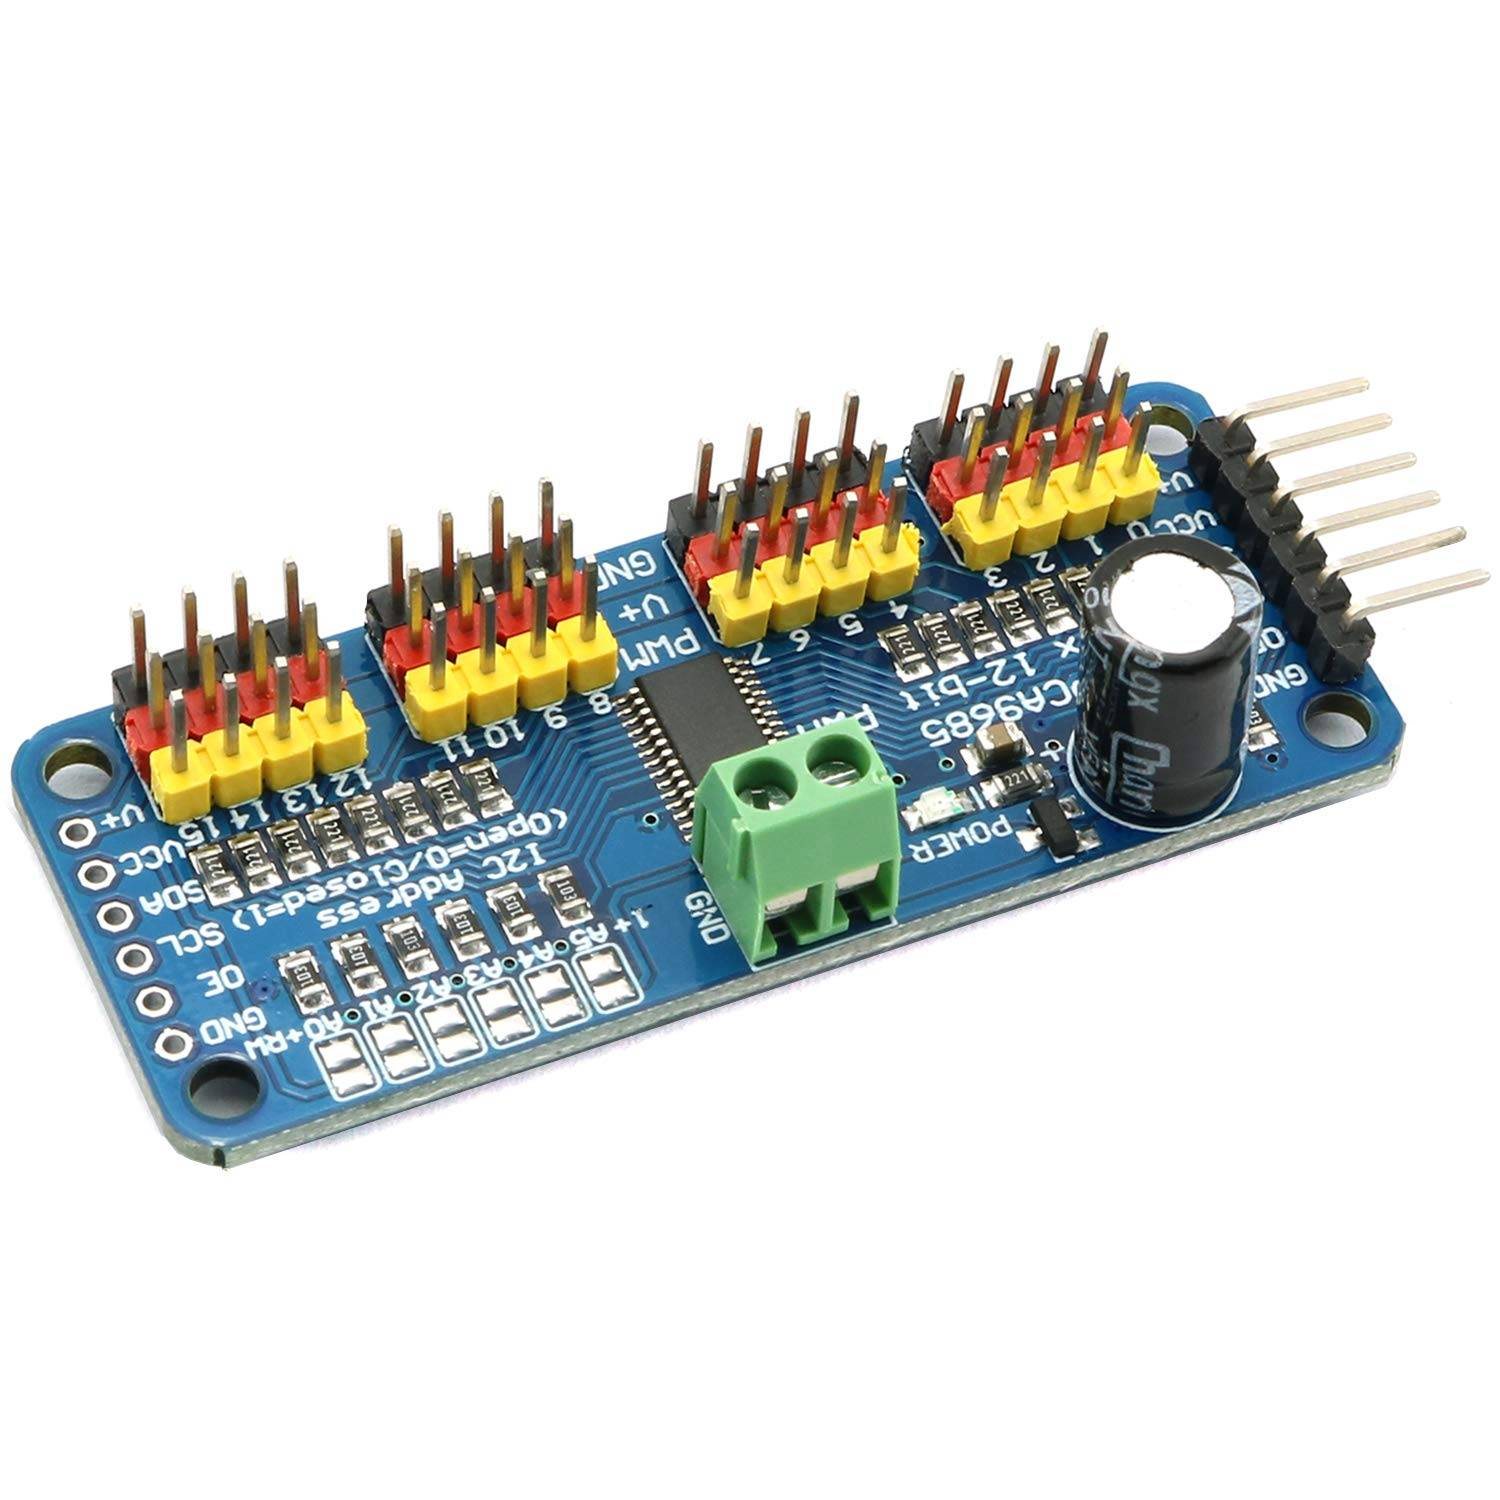
\includegraphics[width=0.5\textwidth]{pca9685}
		\caption{PCA 9685}
		\label{pca9685}
	\end{center}
\end{figure}

\subsection{Выбор инерционного датчика}\label{C4_4_3}

В ходе разработки прототипа возникла проблема с регулированием управления. Главной причиной послужило какое-либо отсутствие обратной связи у сервоприводов, о чем уже упоминалось в разделе \ref{C4_4_1}. Были предложены несколько решений данной проблемы:
\begin{enumerate}
	\item Модификация каждой платы управления сервоприводом;
	\item Подключение гироскопа акселерометра к каждому сервоприводу;
	\item Установка гироскопа акселерометра на корпусе робота.
\end{enumerate}
Первый вариант заключается в демонтаже каждого привода и прямого подключения в выходной сигнал управляющий платы.\newline 
Преимущества:
\begin{itemize}
 	\item Получение реальных углов поворота, которые принимают валы двигателей.
 	\item Нет необходимости корректировать уравнения кинематики.
 	\item Нет необходимости дополнительных вычислений, достаточно учитывать ошибку между реальным и идеальным значением на каждом шаге.
\end{itemize}
Недостатки:
\begin{itemize}
	\item Восемь аналоговых подключений.
	\item OrangePi не поддерживает аналоговые порты.
	\item Требуются дополнительные преобразовательные модули.
	\item Необходимо фильтровать данные.
\end{itemize}
Вывод:
Данное решение, не смотря на его простоту, не является подходящим, так как нет возможности его корректной реализации.
\newline


Второй метод представляет из себя снятие отклонения углов напрямую, преобразуя снятые данные с гироскопа акселерометра. Далее учитывать полученную ошибку на каждом шаге.
\newline
Преимущества:
 \begin{itemize}
 	\item Получение реальных углов поворота, которые принимают голень и бедро робота.
 	\item Нет необходимости корректировать уравнения кинематики.
 	\item Нет необходимости лишних вычислений, достаточно учитывать ошибку между реальным и идеальным значением на каждом шаге.
 	\item Получаемые данные цифровые. Это позволяет их легко обрабатывать.
 \end{itemize}
Недостатки:
\begin{itemize}
\item Гироскоп акселерометр имеет свойство накапливать ошибку. В данном случае их 8 штук, как следствие, низкая точность.
\item Восемь цифровых подключений.
\item Сложность калибровки каждого датчика отдельно.
\item Требуется дополнительный модуль "сплиттер" для подключения более двух гироскопов акселерометров.
\item Необходимо фильтровать данные.
\end{itemize}
Вывод:
Данное решение не является подходящим, так как необходимы дополнительные модули для работы с гироскопами акселерометрами в количестве более двух штук. Также существенной сложностью является калибровка большого количества датчиков и поддержание необходимой точности вычислений.
\newline


Третий метод заключается в креплении гироскопа акселерометра на корпусе робота и последующего регулировании его отклонения в плоскостях тангажа и крена, тем самым соблюдая условие комфортабельности походки, то есть реализация поступательного, равномерного и прямолинейного движения корпуса.
\newline
Преимущества:
\begin{itemize}
	\item Подключение всего одного датчика.
	\item Малые затраты на реализацию.
	\item Компенсация отклонений корпуса в плоскостях тангажа и рысканья.
	\item Получаемые данные цифровые. Это позволяет их легко обрабатывать.
\end{itemize}
Недостатки:
\begin{itemize}
	\item Необходимо корректировать уравнения кинематики.
	\item Необходимо фильтровать данные
	\item Получаемые данные цифровые. Это позволяет их легко обрабатывать.
\end{itemize}

В настоящей работе выбран третий вариант, реализация которого подробна описана в разделе \ref{C5_3}. В качестве инерционного датчика выбран модуль MPU6050 (рисунок \ref{mpu6050}).
\newpage
\begin{figure}[h!]
	\begin{center}
		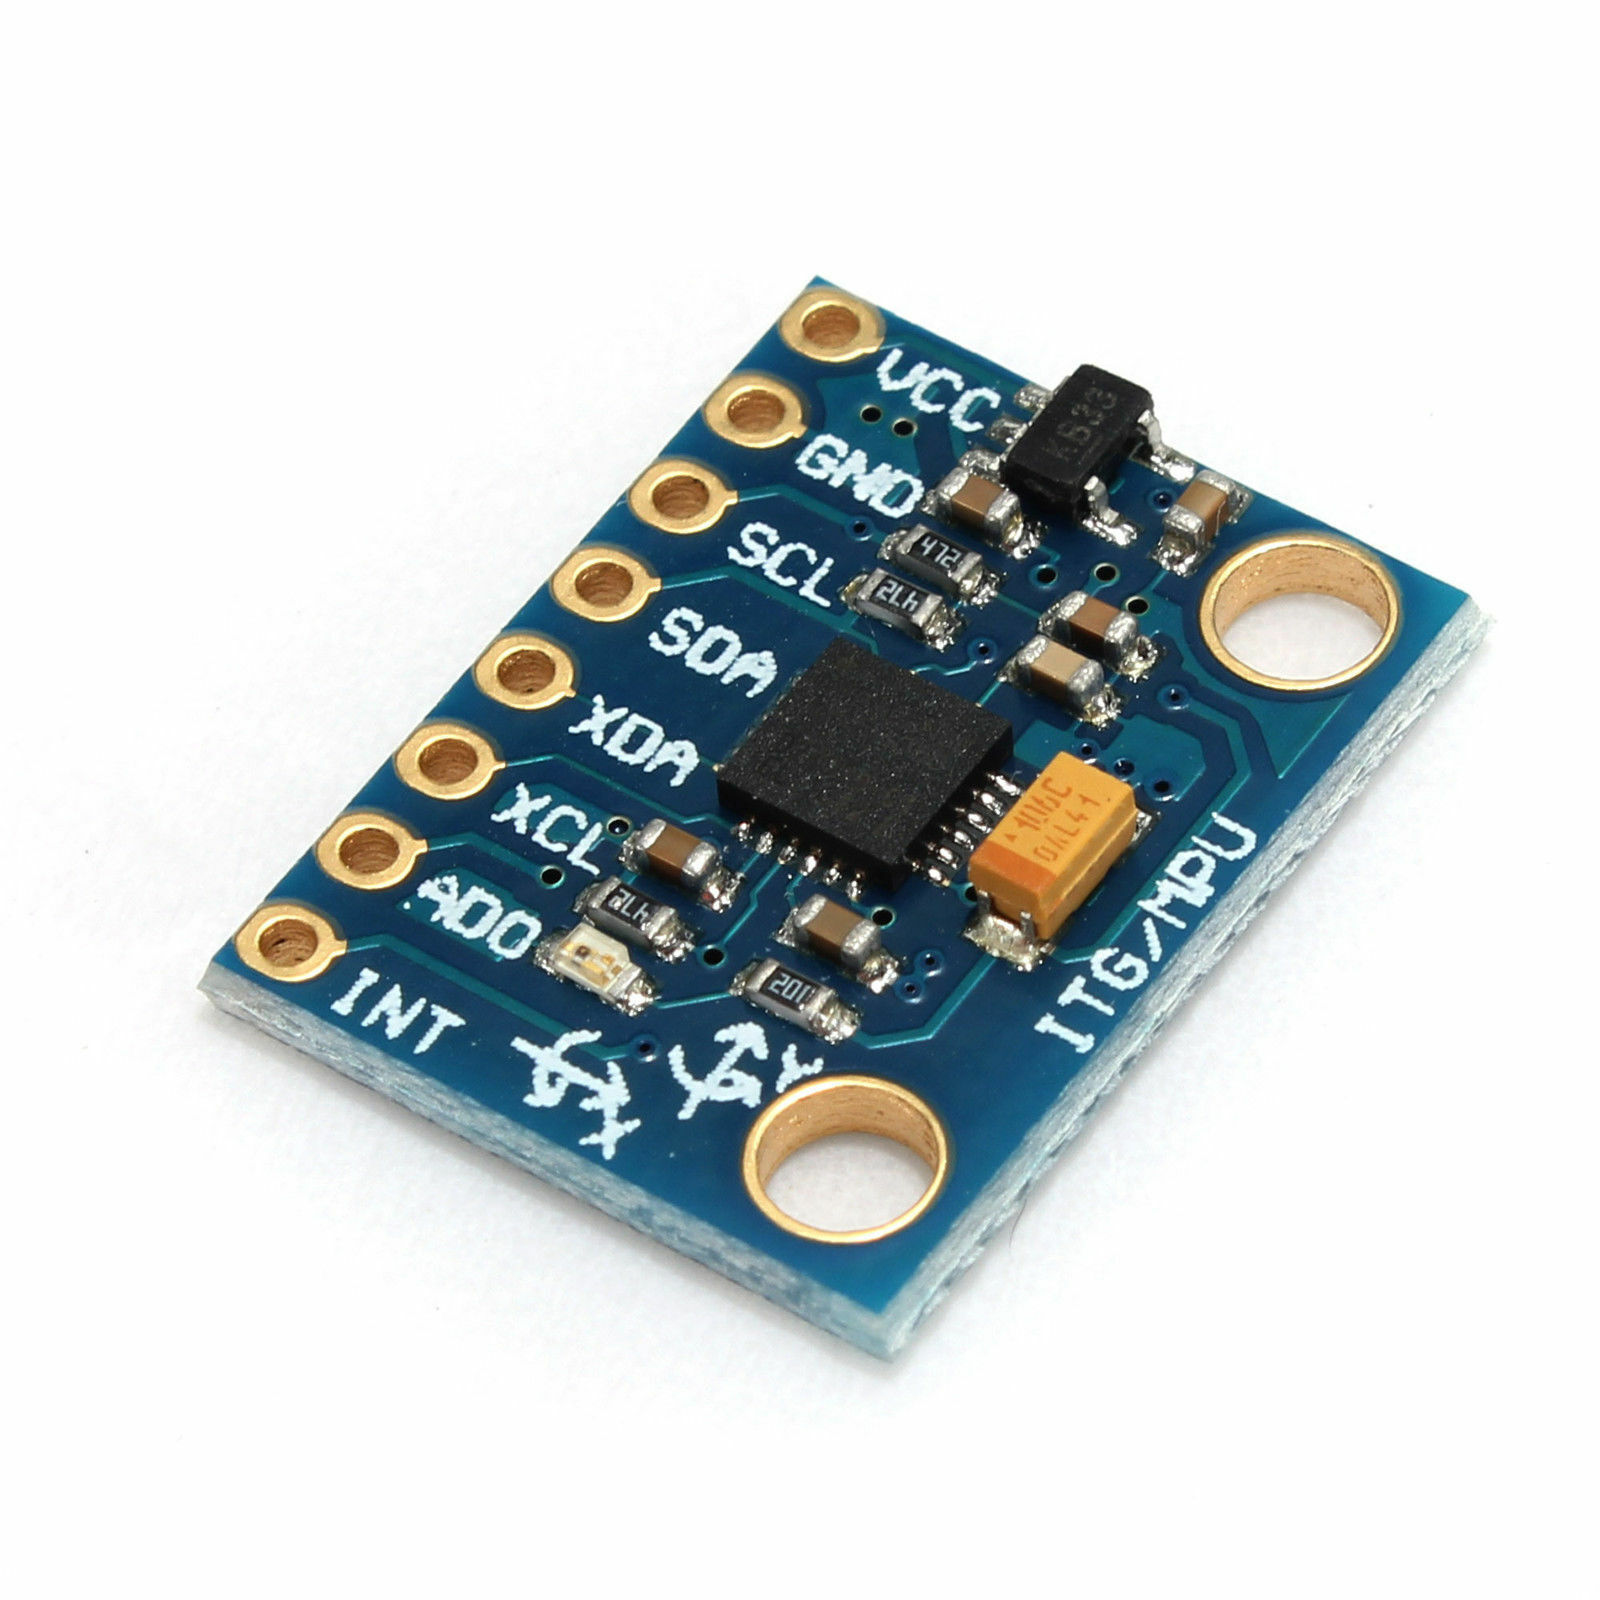
\includegraphics[width=0.5\textwidth]{mpu6050}
		\caption{MPU 6050}
		\label{mpu6050}
	\end{center}
\end{figure}

\subsection{Выбор источника питания}\label{C4_4_4}
Источник питания необходимо выбирать опираясь на определенные критерии. Опишем их в порядке значимости:
\begin{itemize}
	\item Высокая токоотдача для нормальной работы сервоприводов.
	\item Большая емкость для продолжительной работы.
	\item Малый вес, чтобы не увеличивать нагрузку на двигатели.
	\item Быстрая зарядка.
\end{itemize}

Таким свойствам удовлетворяет большинство Li-Po аккумуляторов, в настоящей работе была выбрана модель Spard Li-Po 3200mAh (рисунок \ref{lipo}).
\begin{figure}[h!]
	\begin{center}
		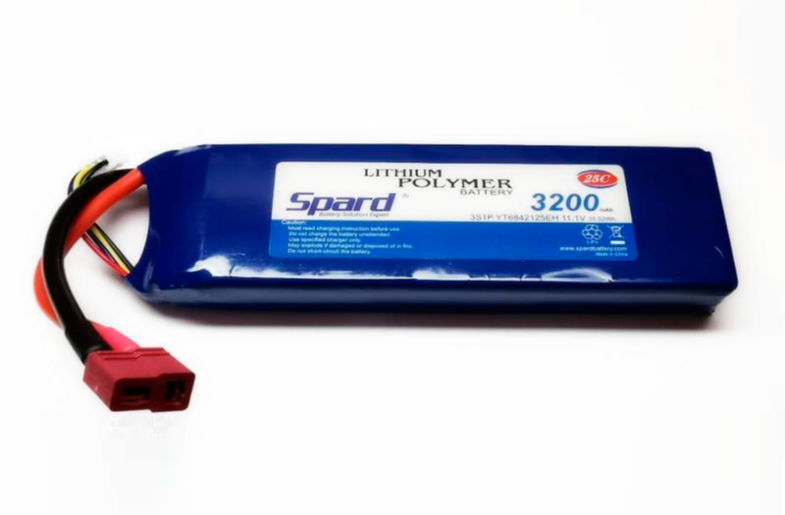
\includegraphics[width=0.5\textwidth]{lipo}
		\caption{Li-Po аккумулятор емкостью 3200 мАч}
		\label{lipo}
	\end{center}
\end{figure}
Этот тип аккумулятора получил широкое распространение благодаря своим высоким характеристикам производительности и компактности. Тип аккумуляторов Li-Po может хранить больше энергии, чем другие типы компактных источников питания, это означает, что он может работать дольше на одном заряде, что делает его идеальным для устройств, которые требуют высокой производительности и долгого времени работы. Однако, как и все, Li-Po аккумуляторы имеют некоторые недостатки. В частности, он может быть более чувствителен к перезарядке, чем другие типы аккумуляторов.Также при возможном коротком замыкании, подключенные элементы имеют высокий шанс на полный выход из строя из-за высокого порога токоотдачи. 

%\textbf{Результаты проектирования и сборки} 
\subsection{Результаты проектирования и сборки}\label{C4_4_5}

Финальный итог сборки робота по описанным выше твердотельным чертежам c перечисленными комплектующими представлен на  рисунках \ref{side}, \ref{back}, \ref{top}. Полная схема подключения электронных компонентов (см. Приложение Б).
\newpage
\begin{figure}[h!]
	\begin{center}
		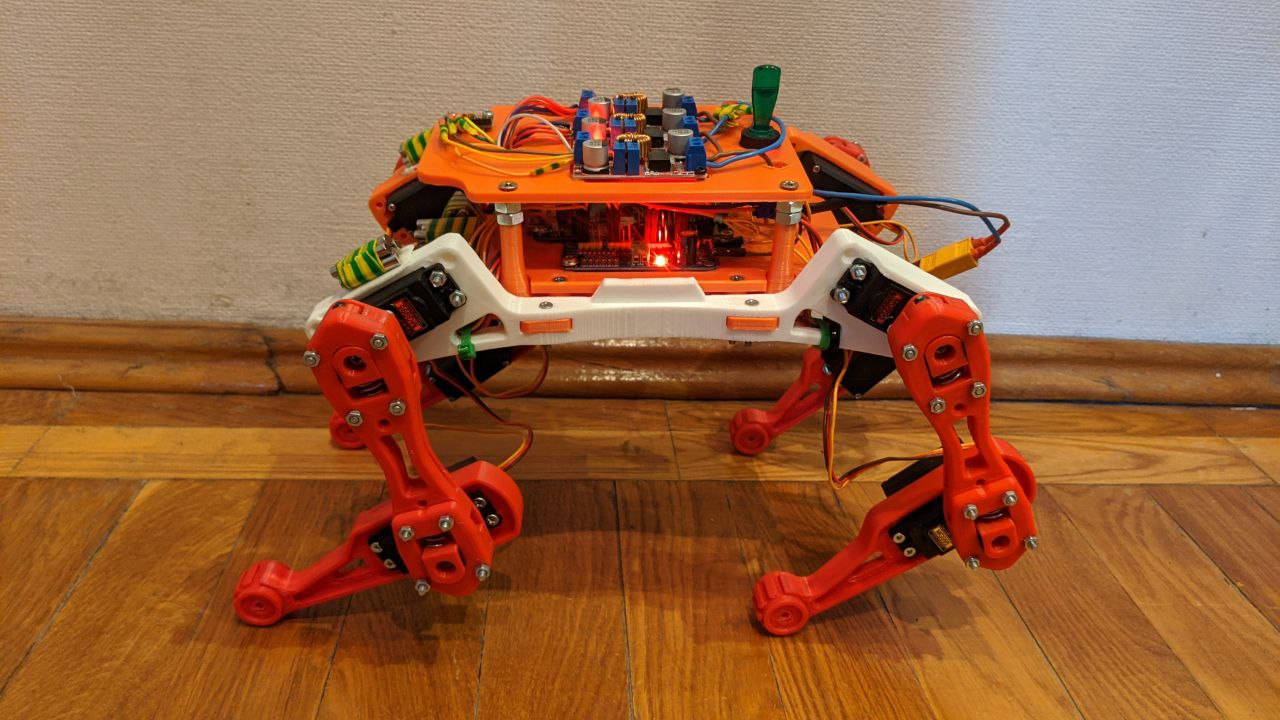
\includegraphics[width=0.9\textwidth]{side}
		\caption{Собранный прототип робота - вид сбоку}
		\label{side}
	\end{center}
\end{figure}

\begin{figure}[h!]
	\begin{center}
		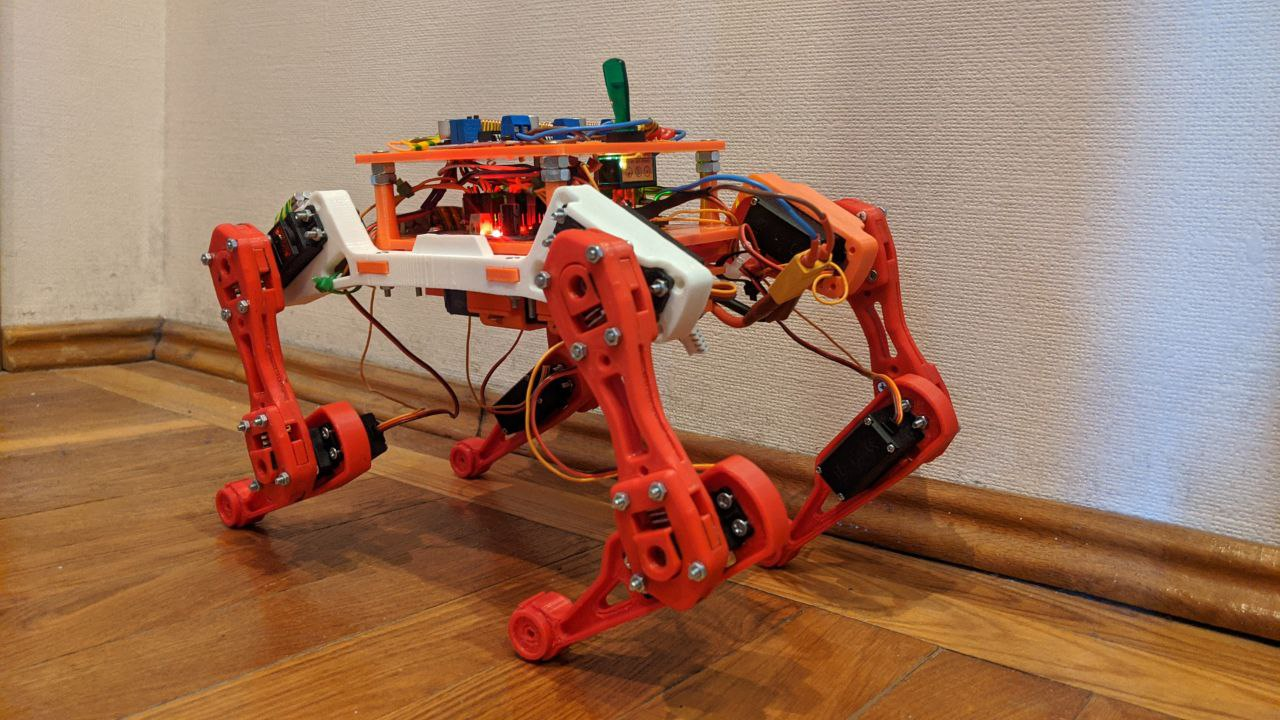
\includegraphics[width=0.9\textwidth]{back}
		\caption{Собранный прототип робота - вид сзади}
		\label{back}
	\end{center}
\end{figure}
\newpage
\begin{figure}[h!]
	\begin{center}
		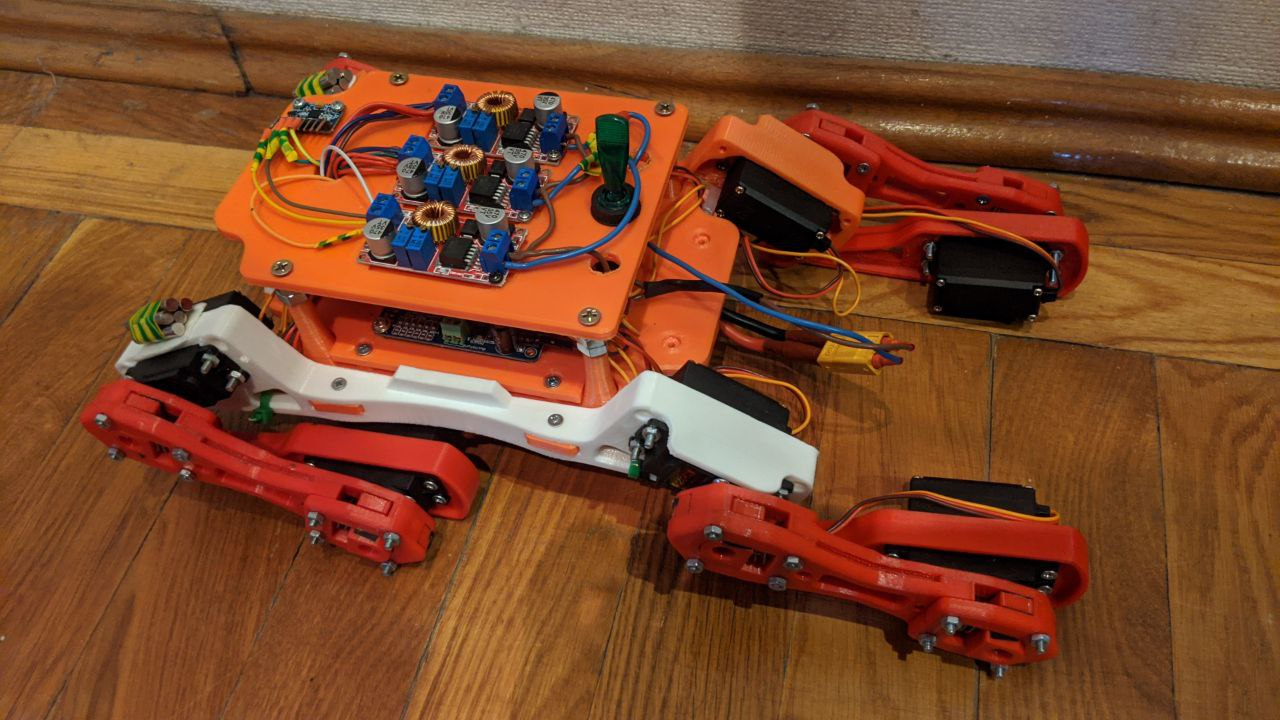
\includegraphics[width=0.9\textwidth]{top}
		\caption{Собранный прототип робота - вид сверху}
		\label{top}
	\end{center}
\end{figure}
	\newpage
	\newpage
\begin{center}
	\textbf{\large ГЛАВА 5 \\ Разработка ПО}
\end{center}
\refstepcounter{chapter}


% \section*{}
\addcontentsline{toc}{chapter}{ГЛАВА 5}
\section{Общая архитектура}\label{C5_1}

Все взаимодействия комплектующих из пунктов \ref{C4_4_1} - \ref{C4_4_5} происходят путем отправки низкоуровневых комманд из миникомпьютера Orange Pi в соответствующие модули. Команды формируются с помощью программного обеспечения, написанного на высокоуровневом языке Python 3. Данный язык был выбран в связи с наличием динамической типизации, богатой библиотекой для математических вычислений и большой существующей кодовой базой, что позволяет быстро писать прототипы для тестирования. На рисунке \ref{arch} показана структура управления роботом.

\begin{figure}[h!]
	\begin{center}
		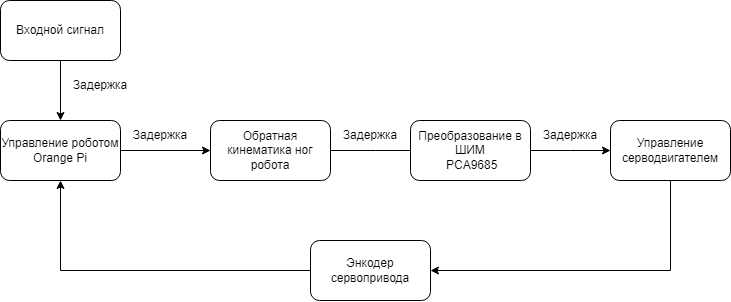
\includegraphics[width=1\textwidth]{arch}
		\caption{Структурная схема управления роботом}
		\label{arch}
	\end{center}
\end{figure}

Система управления роботом интерпретирует входные данные от устройства ввода и преобразует их в траекторию ходьбы для последующего позиционирования тела робота. Блоки обратной кинематической преобразуют координаты ноги в положения сервопривода.

\section{Обратная связь с помощью гироскопа}\label{C5_2}

Главным недостатком такой структуры управления --- недоступность реальных значений углов поворота двигателя, как уже упоминалось в разделе \ref{C4_4_1}, в следствие чего невозможно контролировать ошибку между идеальными и реальными значениями углов вала серводвигателя. Были предложены несколько решений данной проблемы:
\begin{enumerate}
	\item Модификация каждой платы управления сервоприводом;
	\item Подключение гироскопа акселерометра к каждому сервоприводу;
	\item Установка гироскопа акселерометра на корпусе робота.
\end{enumerate}
Первый вариант заключается в демонтаже каждого привода и прямого подключения в выходной сигнал управляющий платы.\newline 
Преимущества:
\begin{itemize}
	\item Получение реальных углов поворота, которые принимают валы двигателей.
	\item Нет необходимости корректировать уравнения кинематики.
	\item Нет необходимости дополнительных вычислений, достаточно учитывать ошибку между реальным и идеальным значением на каждом шаге.
\end{itemize}
Недостатки:
\begin{itemize}
	\item Восемь аналоговых подключений.
	\item OrangePi не поддерживает аналоговые порты.
	\item Требуются дополнительные преобразовательные модули.
	\item Необходимо фильтровать данные.
\end{itemize}
Вывод:
Данное решение, не смотря на его простоту, не является подходящим, так как нет возможности его корректной реализации.
\newline


Второй метод представляет из себя снятие отклонения углов напрямую, преобразуя снятые данные с гироскопа акселерометра. Далее учитывать полученную ошибку на каждом шаге.
\newline
Преимущества:
\begin{itemize}
	\item Получение реальных углов поворота, которые принимают голень и бедро робота.
	\item Нет необходимости корректировать уравнения кинематики.
	\item Нет необходимости лишних вычислений, достаточно учитывать ошибку между реальным и идеальным значением на каждом шаге.
	\item Получаемые данные цифровые. Это позволяет их легко обрабатывать.
\end{itemize}
Недостатки:
\begin{itemize}
	\item Гироскоп акселерометр имеет свойство накапливать ошибку. В данном случае их 8 штук, как следствие, низкая точность.
	\item Восемь цифровых подключений.
	\item Сложность калибровки каждого датчика отдельно.
	\item Требуется дополнительный модуль ``сплиттер'' для подключения более двух гироскопов акселерометров.
	\item Необходимо фильтровать данные.
\end{itemize}
Вывод:
Данное решение не является подходящим, так как необходимы дополнительные модули для работы с гироскопами акселерометрами в количестве более двух штук. Также существенной сложностью является калибровка большого количества датчиков и поддержание необходимой точности вычислений.
\newline


Третий метод заключается в креплении гироскопа акселерометра на корпусе робота и последующего регулирования его отклонений в плоскостях тангажа и крена, тем самым соблюдая условие комфортабельности походки, то есть реализация поступательного, равномерного и прямолинейного движения корпуса.
\newline
Преимущества:
\begin{itemize}
	\item Подключение всего одного датчика.
	\item Малые затраты на реализацию.
	\item Компенсация отклонений корпуса в плоскостях тангажа и рысканья.
	\item Получаемые данные цифровые. Это позволяет их легко обрабатывать.
\end{itemize}
Недостатки:
\begin{itemize}
	\item Необходимо корректировать уравнения кинематики.
	\item Необходимо фильтровать данные
	\item Получаемые данные цифровые. Это позволяет их легко обрабатывать.
\end{itemize}

\noindent В настоящей работе выбран третий вариант, в таком случае структурная схема управления примет вид (см.рисунок \ref{arch_new}).
\newpage
\begin{figure}[h!]
	\begin{center}
		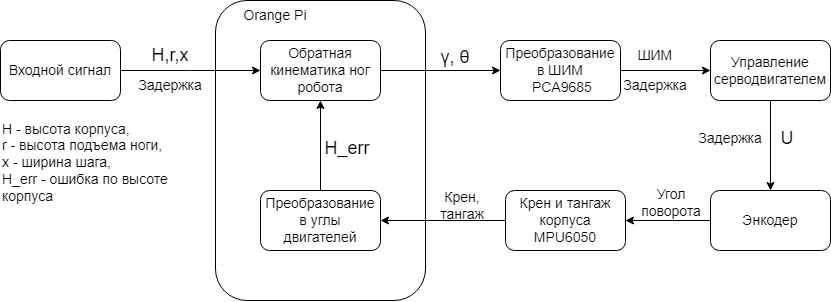
\includegraphics[width=1.2\textwidth,angle=90]{arch_new}
		\caption{Структурная схема управления роботом с обратной связью}
		\label{arch_new}
	\end{center}
\end{figure}
\newpage
\section{Движение робота вперед с обратной связью}\label{C5_3}

Преобразование углов крена и тангажа в углы серводвигателей происходят по алгоритму, описанному ниже:

Для опорный фазы:
\begin{python}
	
    def callculate_step(x_range_step):

		roll_ang,elev_ang = get_pitch_roll() # get data from MPU6050
		elev = np.sin(elev_ang)*body_l//2 # recalculate pitch angle to height
		roll = np.sin(roll_ang)*body_w//2 # recalculate roll angle to height
		y_step=0
		height = drop + elev # include height error (pitch component)
		hip_offset = np.arcsin(elev / body_l) 
		height_slew = np.sqrt(x_range_step**2+(height-y_step)**2)+roll # include height error (roll component) 
		hip_step = 0.5*np.pi - np.arccos(height_slew/(2*self.l1))+np.arctan(x_range_step/(height-y_step)) + hip_offset # conversion to hip servo angle
		knee_step = 2*np.arcsin(height_slew/(2*self.l1)) # conversion to knee servo angle
	
	return np.rad2deg(hip_step), np.rad2deg(knee_step)	
\end{python}

Для свободной фазы аналогично:
\begin{python}
	
    def callculate_skip(x_range_skip,min_delta):
    
		roll_ang,elev_ang = get_pitch_roll() # get data from MPU6050
		elev = np.sin(elev_ang)*body_l//2 # recalculate pitch angle to height
		roll = np.sin(roll_ang)*body_w//2 # recalculate roll angle to height
			
		delta = np.sqrt(self.r**2-min_delta**2)
		y_skip = np.sqrt((self.r**2) - (x_range_skip**2)) - delta
		height = drop + elev # include height error (pitch component)
		hip_offset = np.arcsin(elev / 105)
		height_slew = np.sqrt(x_range_skip**2+(height-y_skip)**2)+roll # include height error (roll component)
		hip_skip = 0.5*np.pi - np.arccos(height_slew/(2*self.l1))+np.arctan(x_range_skip/(height-y_skip)) + hip_offset # conversion to hip servo angle
		knee_skip = 2*np.arcsin(height_slew/(2*self.l1)) # conversion to knee servo angle

	return np.rad2deg(hip_skip),np.rad2deg(knee_skip)
	
\end{python}

Используя данные алгоритмы, получим метрики при движении робота для значений $X_{\text{ш}}$ от $-$50 мм до 50 мм с шагом 1 мм, высотой $h_\text{корп}$ = 150 мм и $r$ = 125 мм. Сравним значения идеальных и реальных углов, полученных с помощью обратной связи.

\begin{figure}[h!]
	\begin{center}
		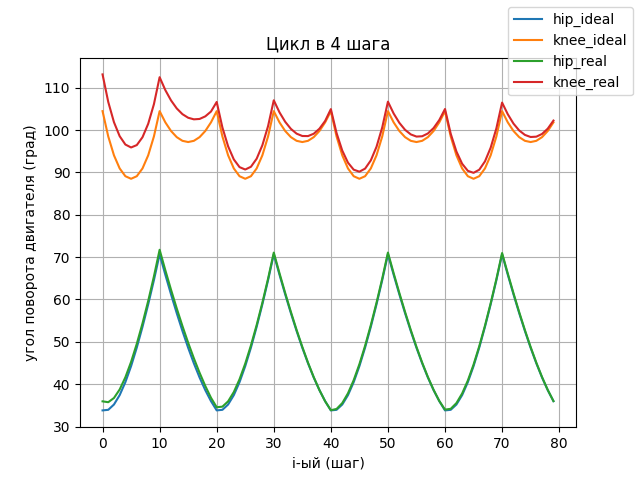
\includegraphics[width=0.9\textwidth]{metrics_servo}
		\caption{Изменение углов двигателей за четыре шага с обратной связью}
		\label{metrics_servo}
	\end{center}
\end{figure}

Исходя из полученного графика можно сделать вывод, что в течение четырех шагов, значения углов на серводвигателях стабилизируются и стремятся к идеальным, что означает работоспособность выбранного метода обратной связи.
\newpage


	\newpage
	\newpage
\begin{center}
	\textbf{ЗАКЛЮЧЕНИЕ}
\end{center}
%\refstepcounter{chapter}
\addcontentsline{toc}{chapter}{ЗАКЛЮЧЕНИЕ}

В рамках работы разработан прототип шагающего робота для образовательных и исследовательских целей. Были составлены чертежи и 3D модели всех составляющих робота, подобраны электрические и логические компоненты, рассчитан худший случай статической нагрузи, исходя из которого была выбрана модель сервоприводов. Исследовано движение стопы шагающего робота, описан процесс решения обратной задачи кинематики для свободного и опорного случая стопы в проблеме о положениях. Произведен синтез походки робота, решена проблема обратной связи реальных углов двигателей с помощью блока гироскопов-акселерометров. Разработано программное обеспечение на языке $Python$ 3 для управления роботом в любой доступной конфигурации, которая ограничена заранее найденной рабочей областью. В кодовой базе описаны протоколы снятия данных и последующего их преобразования, в качестве результата приведены графики реальных и идеальных значений углов поворота двигателей.

Все поставленные цели работы достигнуты, а результат проекта представлен в качестве рабочего прототипа с дистанционным управлением. 


	%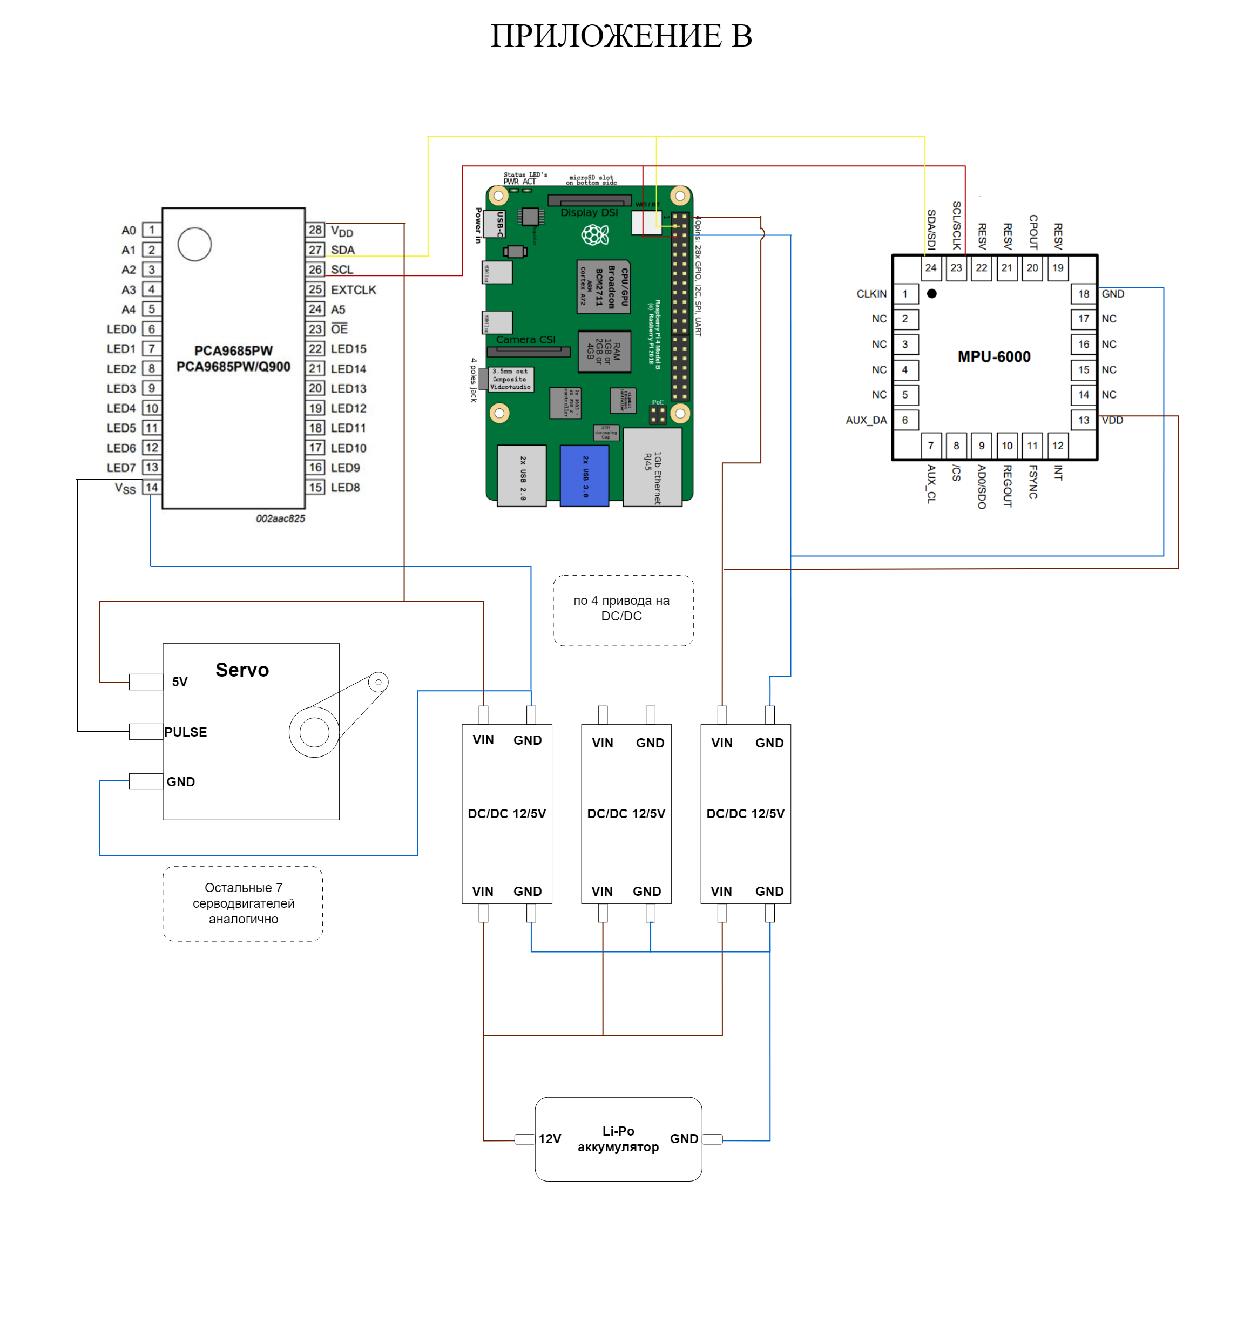
\includepdf[pages={1-1}]{net_scheme.pdf}
	
	\bibliographystyle{unsrt}
	\renewcommand\bibname{\normalsize СПИСОК ИСПОЛЬЗОВАННЫХ ИСТОЧНИКОВ}
	\let\BibEmph=\emph
	\bibliographystyle{ugost2008}  %% стилевой файл для оформления по ГОСТу
	\bibliography{Bak}
	\newpage
	
	\appendix
	\addcontentsline{toc}{chapter}{ПРИЛОЖЕНИЕ А}
	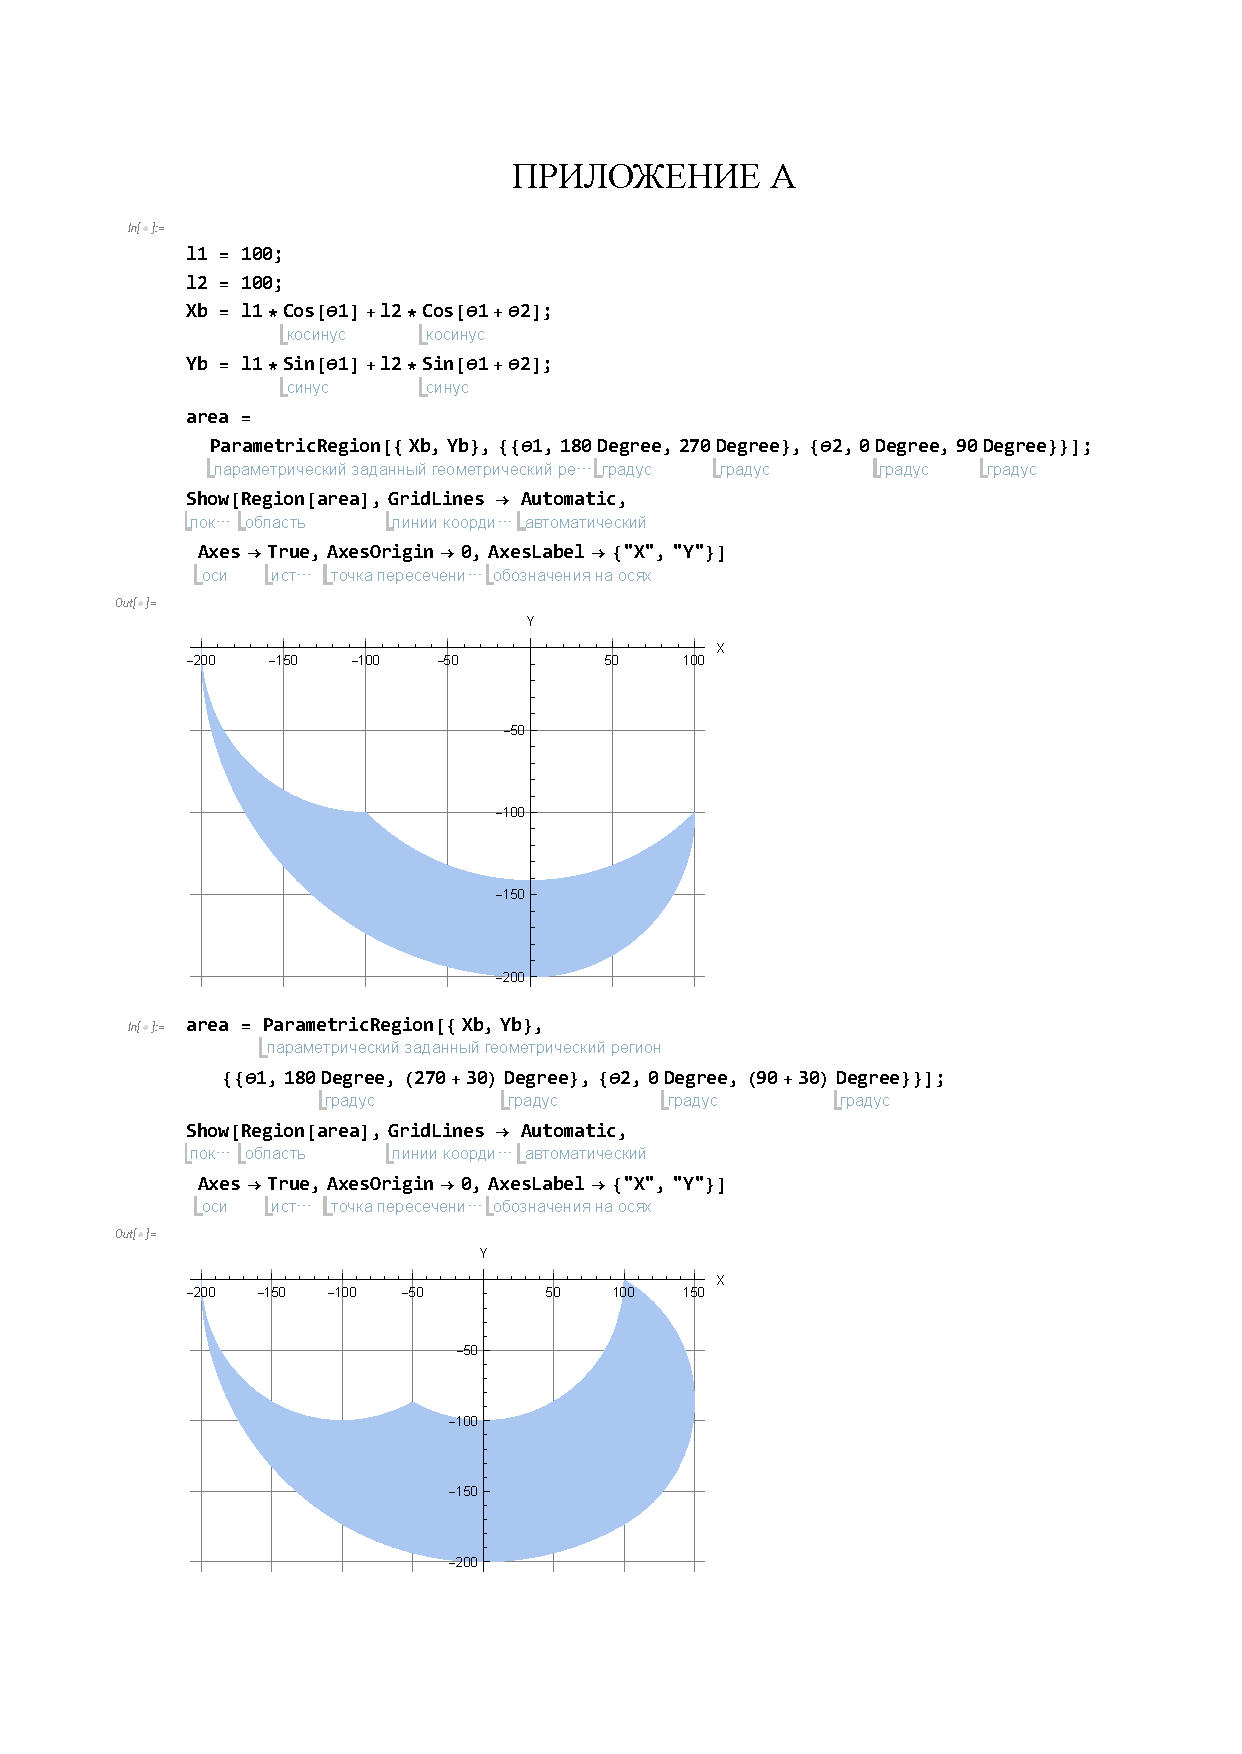
\includepdf[pages=1,pagecommand={}]{work_area.pdf}
	\newpage
	
	\addcontentsline{toc}{chapter}{ПРИЛОЖЕНИЕ Б}
	\KOMAoptions{paper=A3}
	\recalctypearea
	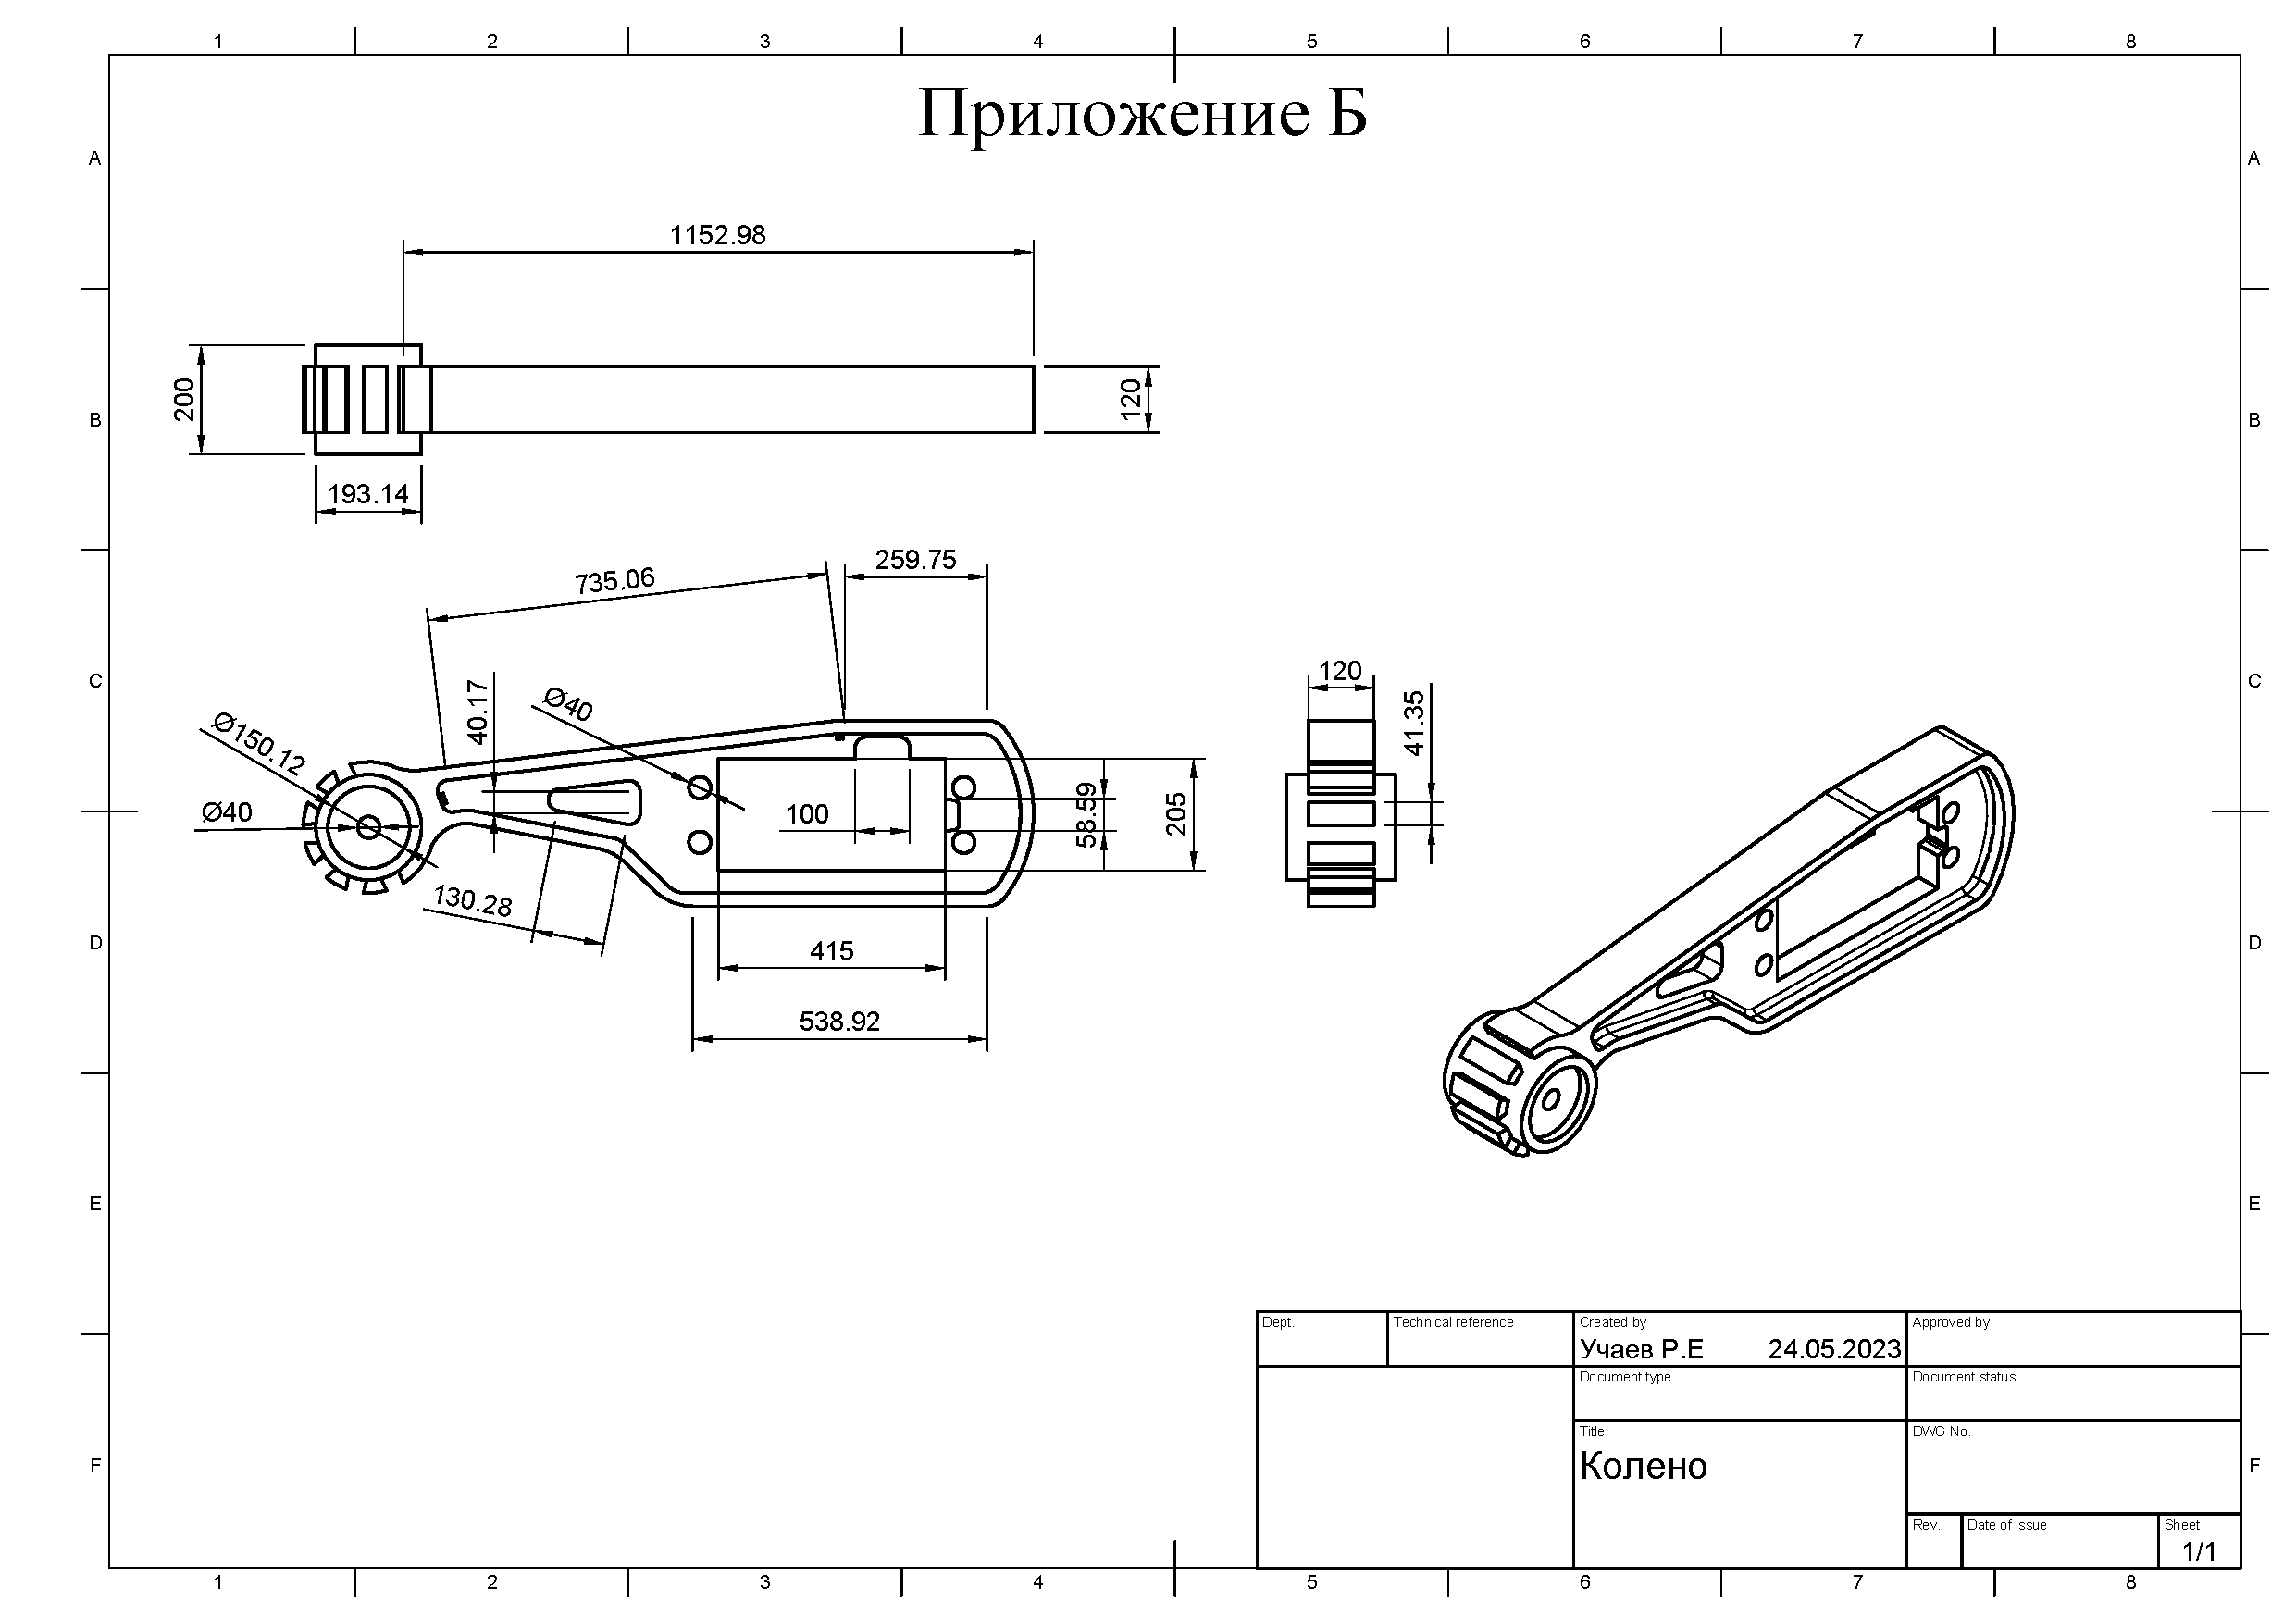
\includepdf[pages=1,angle=90,noautoscale]{knee_draw}
	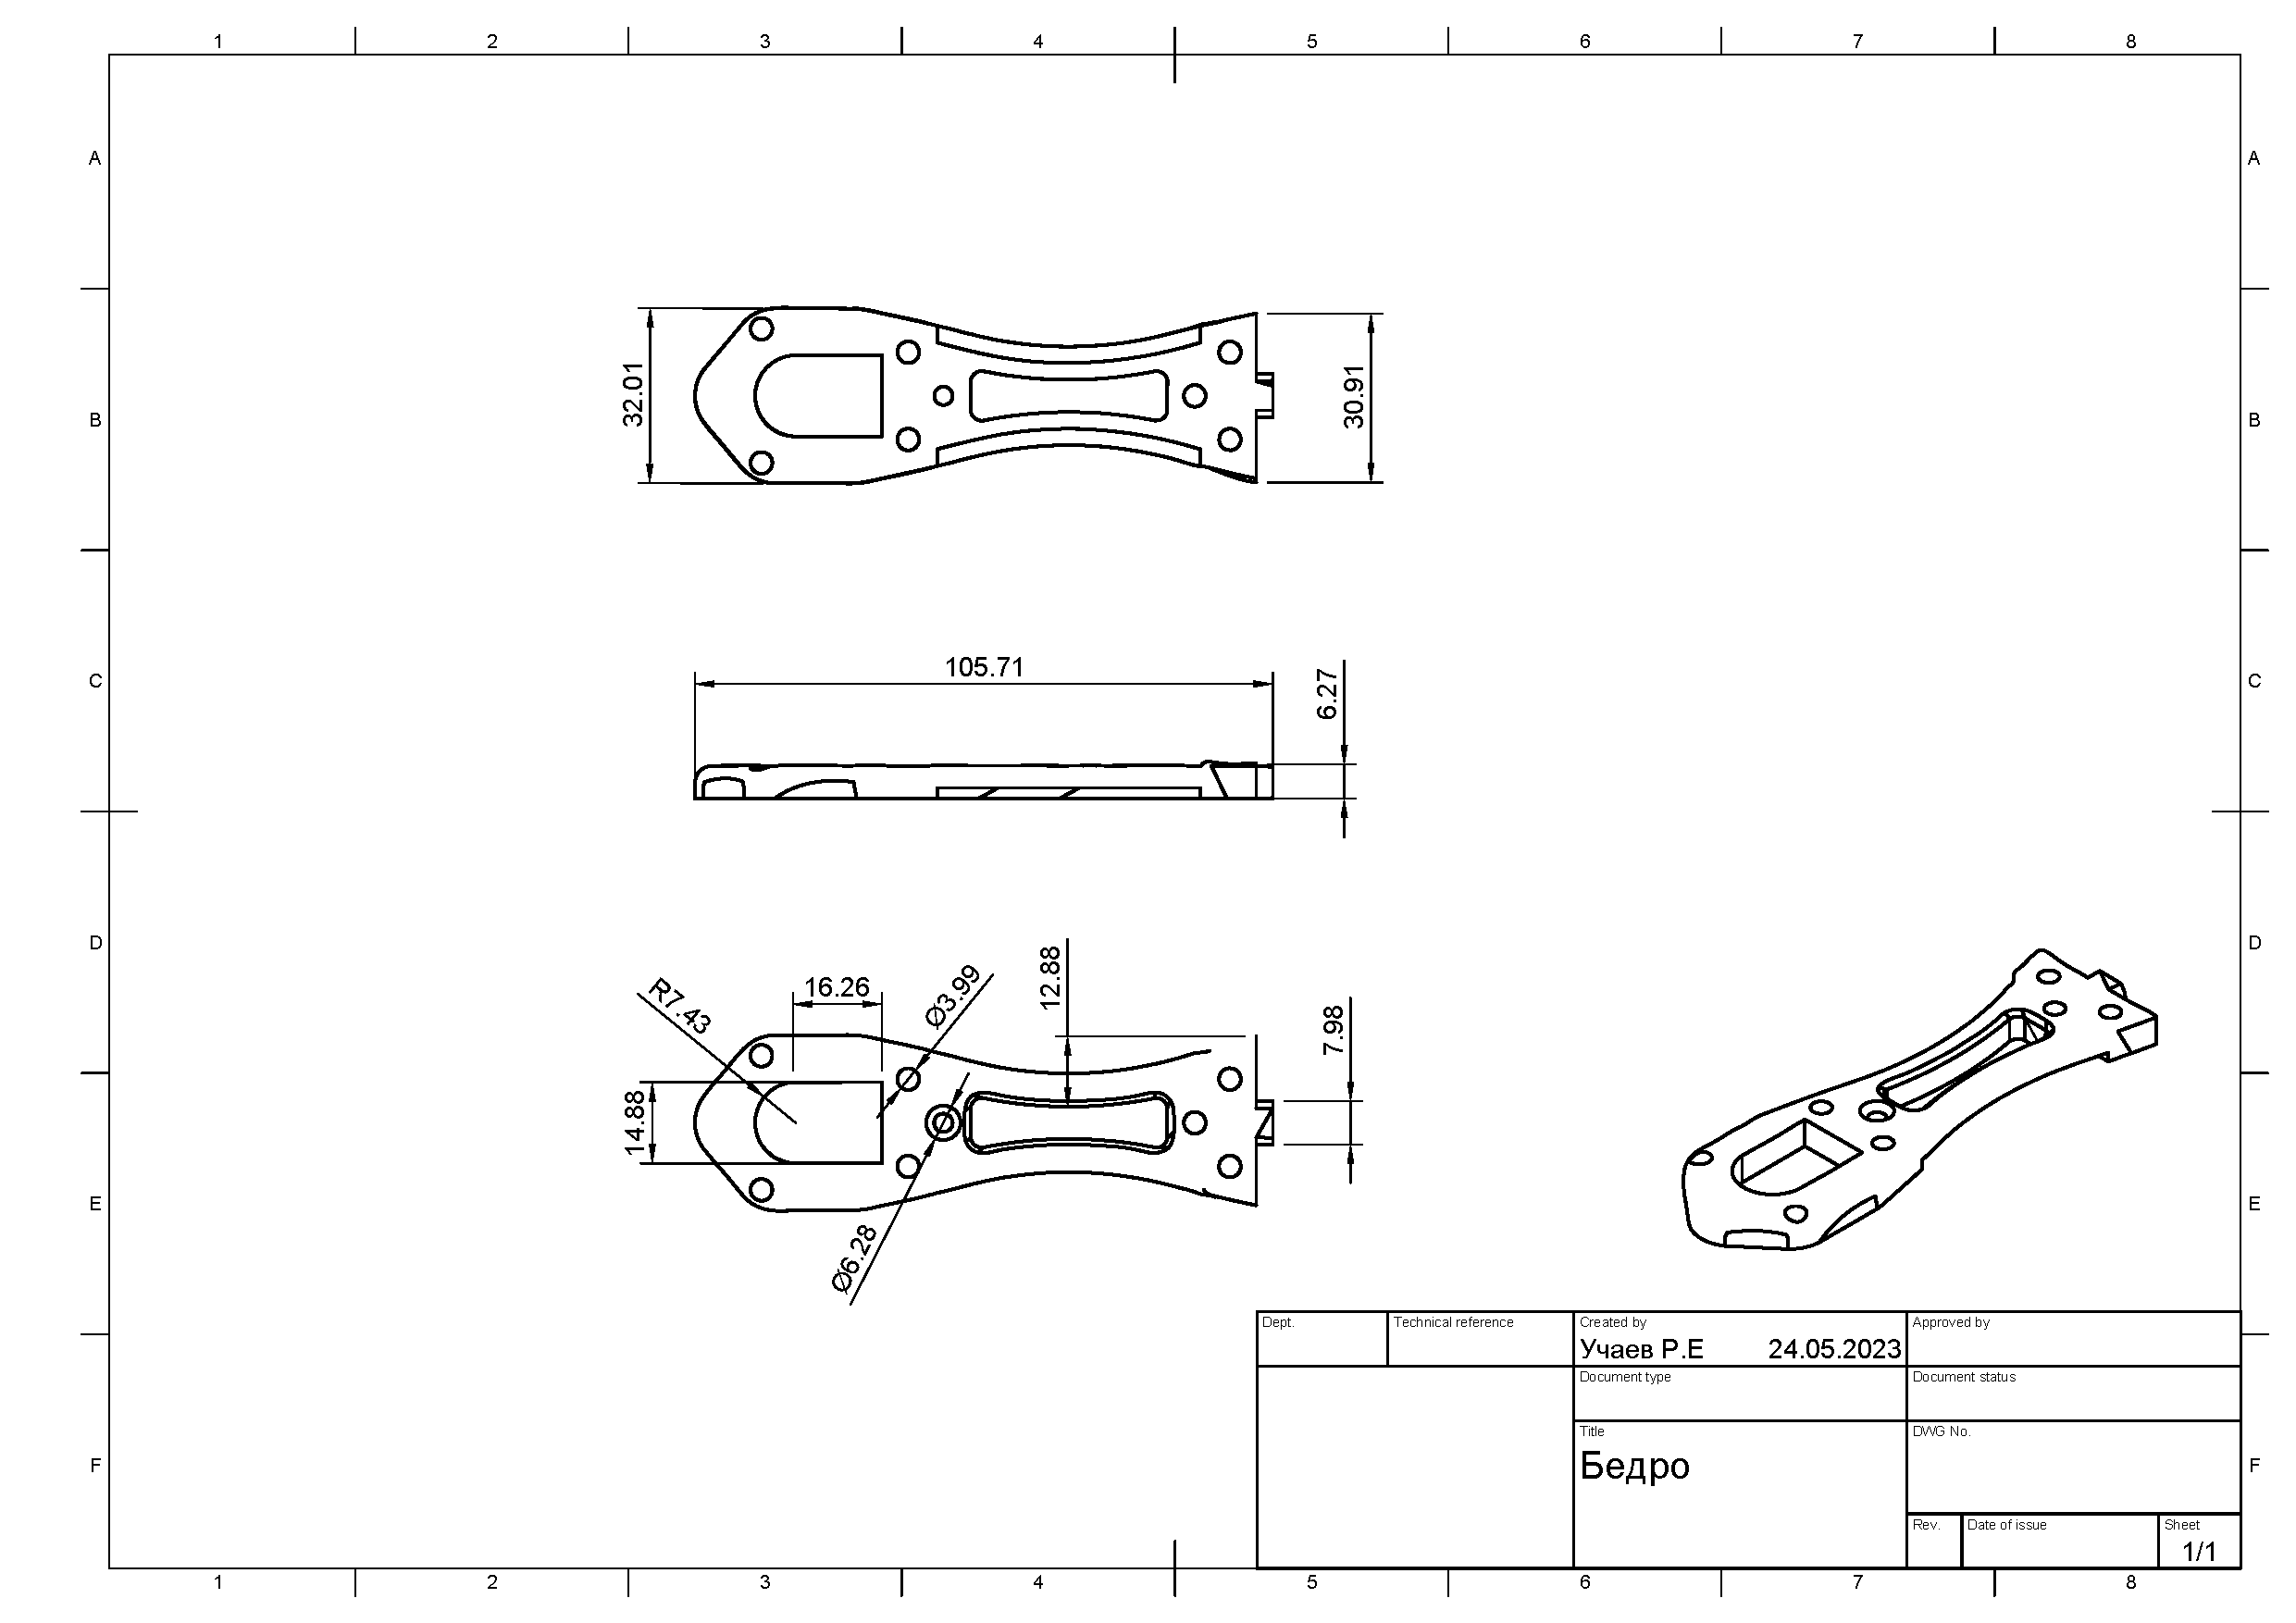
\includepdf[pages=1,angle=90,noautoscale]{hip_draw}
	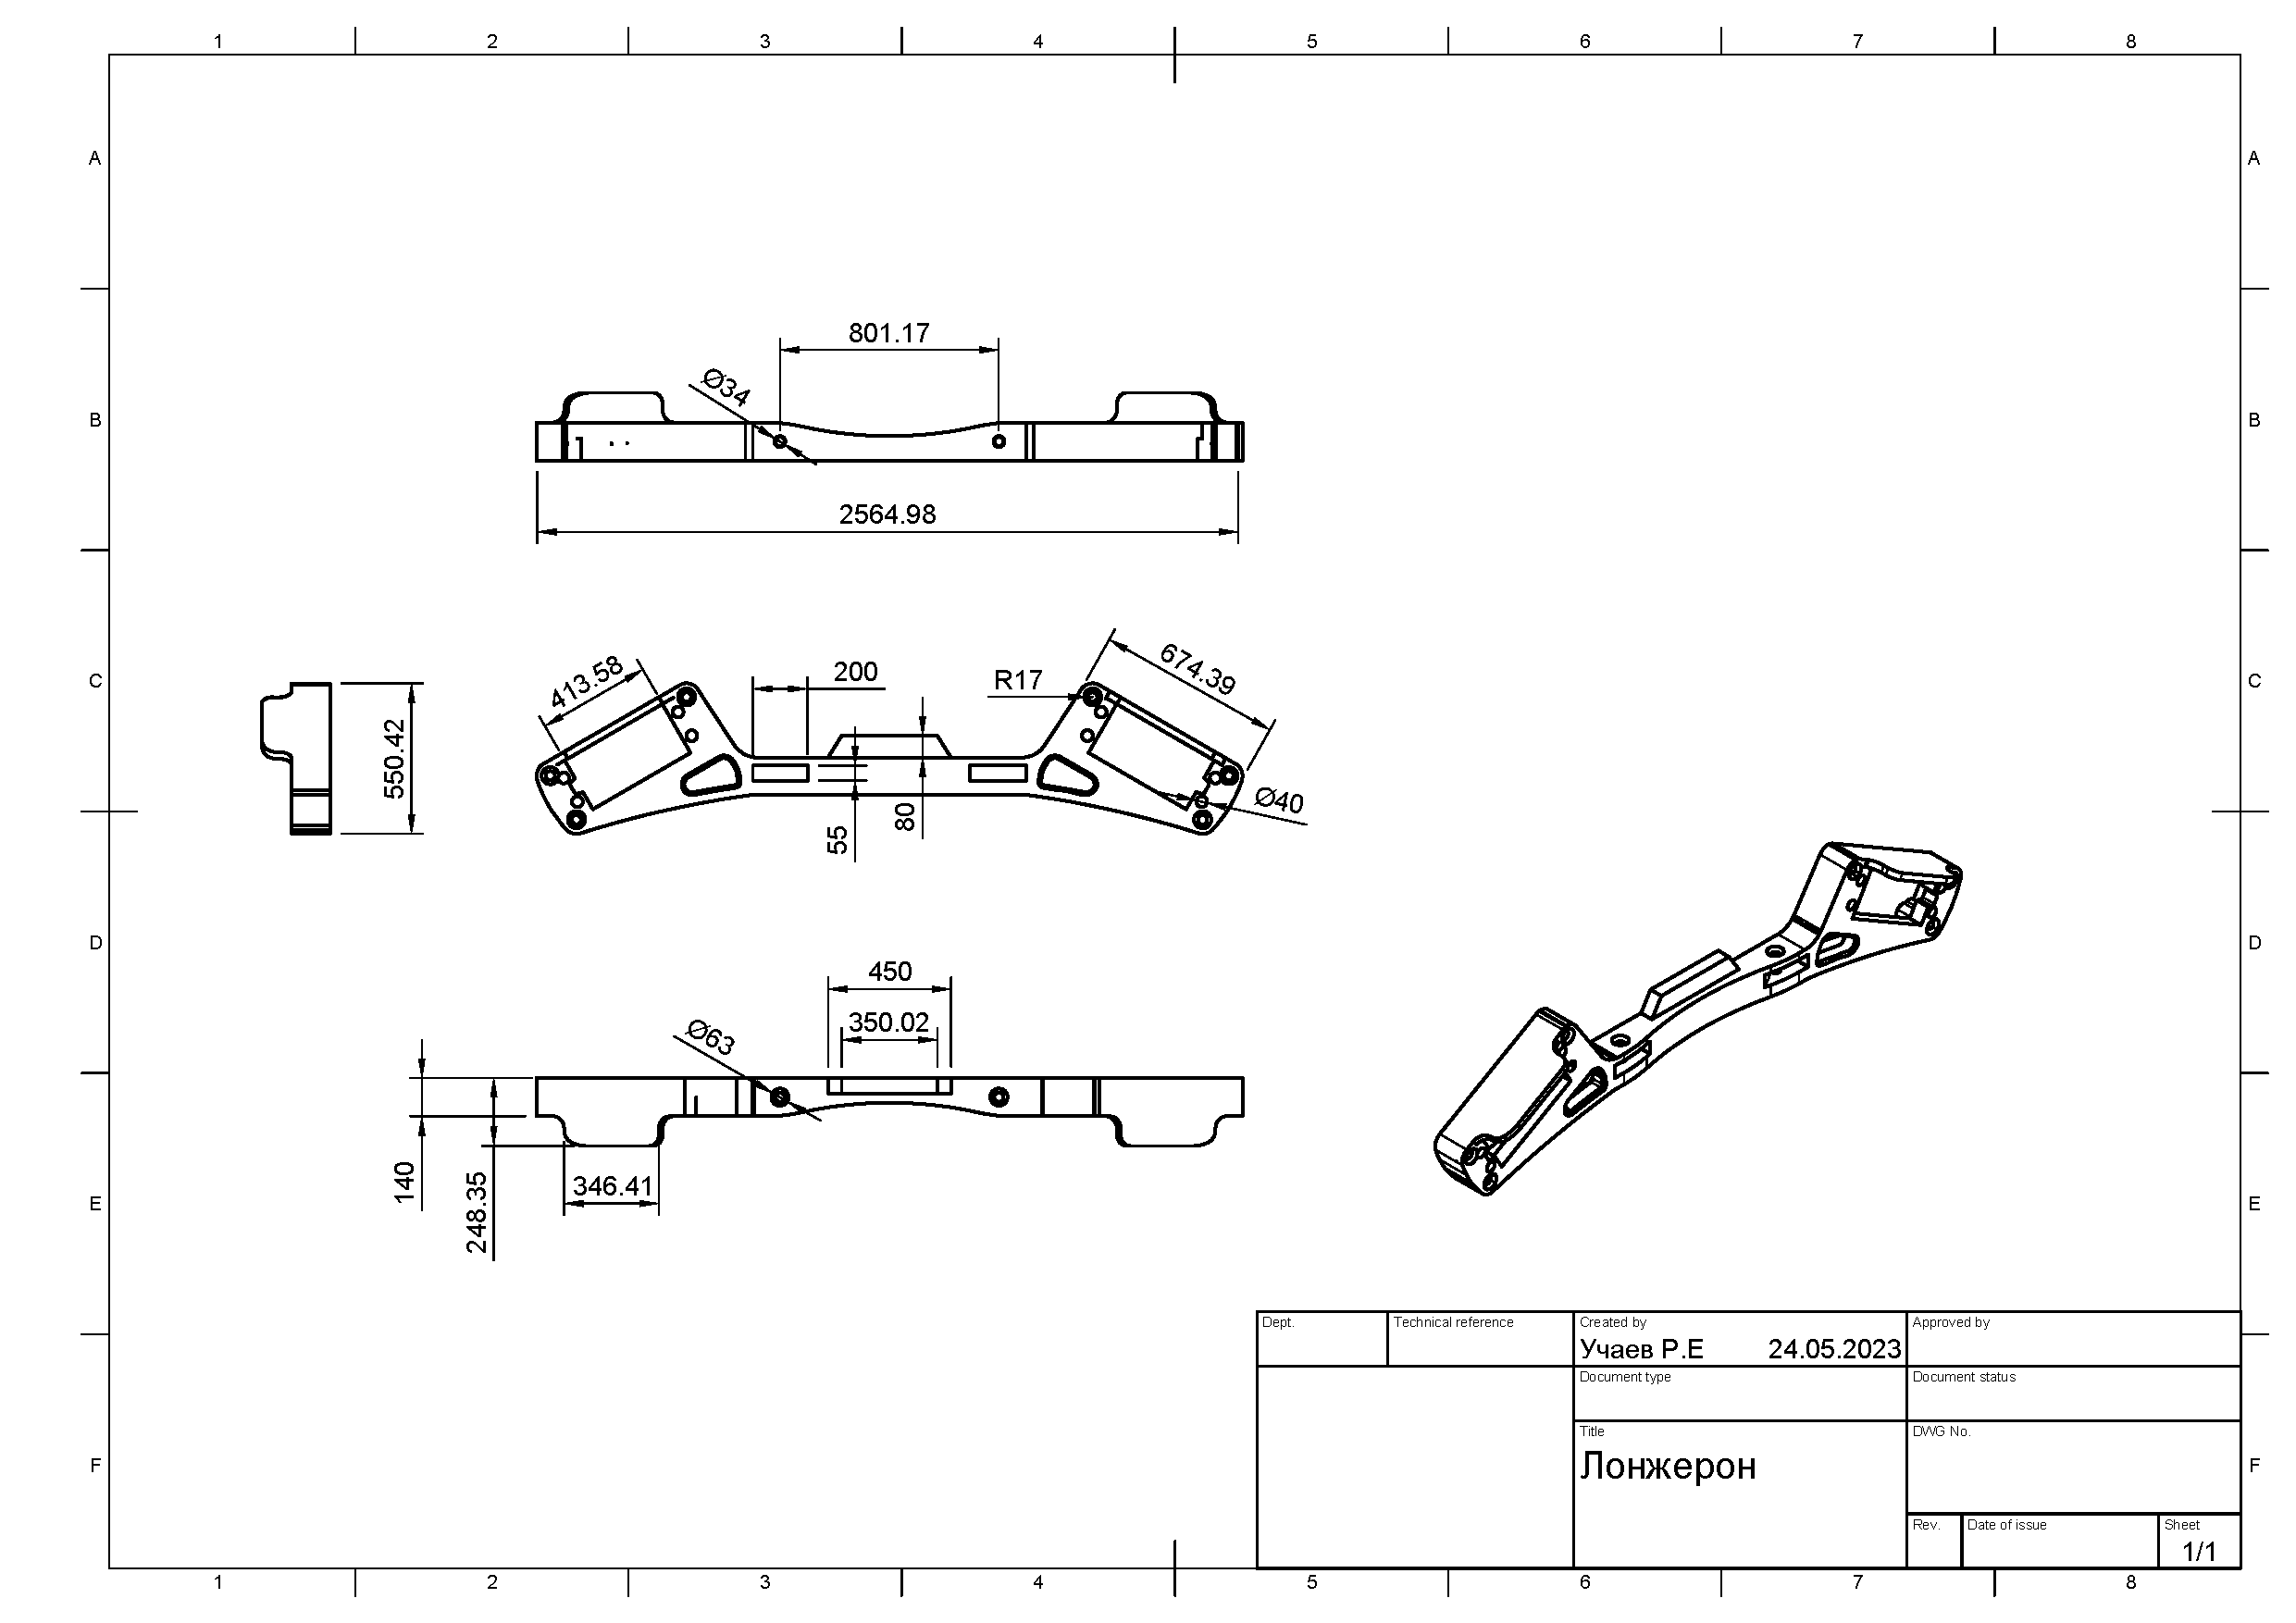
\includepdf[pages=1,angle=90,noautoscale]{longerone_draw}
	
	\KOMAoptions{paper=A4}
	\recalctypearea
	\addcontentsline{toc}{chapter}{ПРИЛОЖЕНИЕ В}
	\begin{center}
		\large\text{ПРИЛОЖЕНИЕ В}
	\end{center}
	
	\begin{figure}[h!]
		\begin{center}
			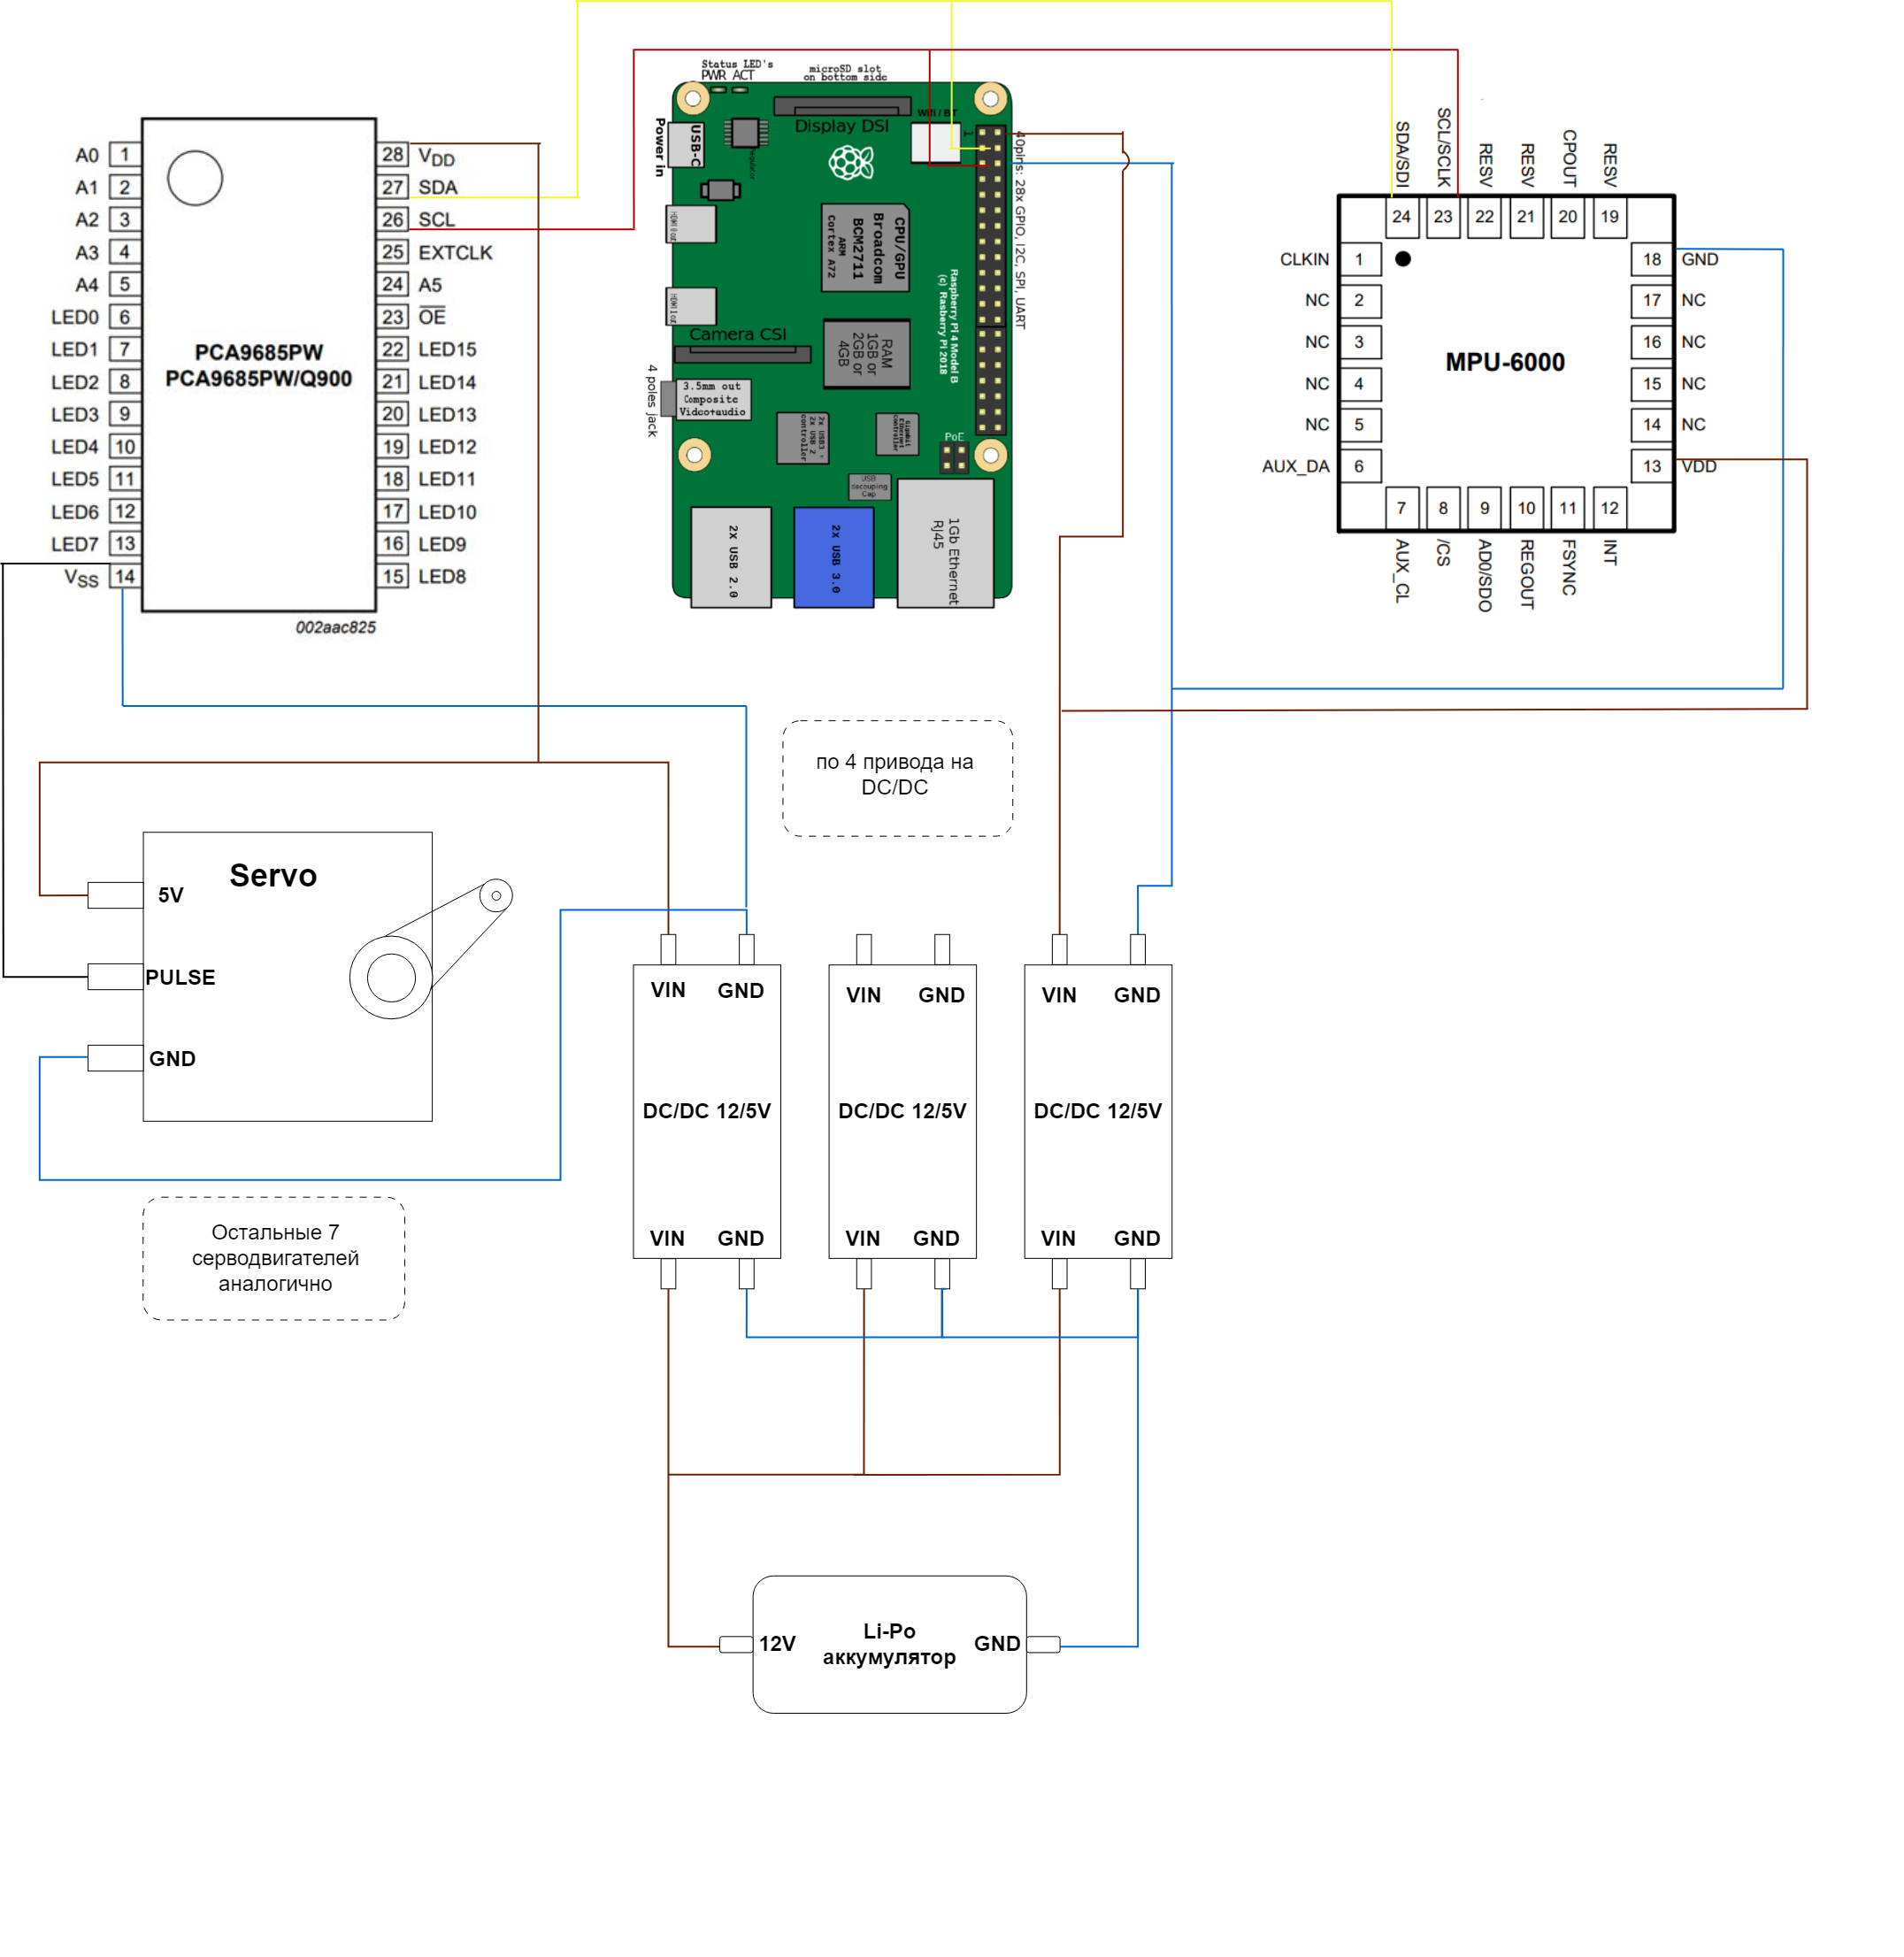
\includegraphics[width=1\textwidth]{net_scheme.png}
		\end{center}
	\end{figure}

	
\end{document}